\documentclass[notitlepage, hidelinks]{article}
\usepackage{natbib}
\usepackage{graphicx}
\usepackage{enumerate}
\usepackage{geometry}
\usepackage{titlesec}
\usepackage{float}
\usepackage{tabularx}
\usepackage[font=footnotesize,labelfont=bf]{caption}
\usepackage{fancyvrb}
\usepackage[ngerman]{babel}
\usepackage{ifxetex,ifluatex}
\usepackage{etoolbox}
\usepackage[svgnames]{xcolor}
\usepackage{tikz}
\usepackage{xcolor}
\usepackage{multirow}
\usepackage{color, colortbl}
\usepackage{wrapfig}
\usepackage{changepage}
\usepackage{listings}
\usepackage[hyphens]{url}
\usepackage{hyperref}
\usepackage{tikz}
\usepackage{caption}
\usepackage{framed}

\newcommand\ytl[2]{
\parbox[b]{16em}{\hfill{\color{black}\bfseries #1}~$\cdots\cdots$~}\makebox[0pt][c]{$\bullet$}\vrule\quad \parbox[c]{14.5cm}{\vspace{10pt}\color{black}\raggedright #2.\\[10pt]}\\[-3pt]
}

\definecolor{Gray}{gray}{0.75}
\definecolor{LightGray}{gray}{0.9}

\definecolor{red}{rgb}{0,0.2,0.701} 
\definecolor{blue}{rgb}{0.023,0.49,0.0117}
\definecolor{green}{rgb}{0,0.8,0}
\definecolor{cyan}{rgb}{0.0,0.38,0.51}
\definecolor{cloudwhite}{rgb}{1, 1, 1}
\definecolor{black}{rgb}{0,0,0}
\definecolor{bluebg}{rgb}{0.05,0.278,0.63}

\lstset{
language=csh,
basicstyle=\footnotesize\ttfamily,
numbers=left,
numberstyle=\tiny,
numbersep=5pt,
tabsize=1,
extendedchars=true,
breaklines=true,
frame=b,
stringstyle=\color{blue}\ttfamily,
showspaces=false,
showtabs=false,
xleftmargin=20pt,
xrightmargin=3pt,
framexleftmargin=17pt,
framexrightmargin=5pt,
framexbottommargin=4pt,
commentstyle=\color{green},
morecomment=[l]{//}, %use comment-line-style!
morecomment=[s]{/*}{*/}, %for multiline comments
showstringspaces=false,
morekeywords={ abstract, event, new, struct,
as, explicit, null, switch,
base, extern, object, this,
bool, false, operator, throw,
break, finally, out, true,
byte, fixed, override, try,
case, float, params, typeof,
catch, for, private, uint,
char, foreach, protected, ulong,
checked, goto, public, unchecked,
class, if, readonly, unsafe,
const, implicit, ref, ushort,
continue, in, return, using,
decimal, int, sbyte, virtual,
default, interface, sealed, volatile,
delegate, internal, short, void,
do, is, sizeof, while,
double, lock, stackalloc,
else, long, static,
enum, namespace, string},
keywordstyle=\color{cyan},
identifierstyle=\color{black},
backgroundcolor=\color{cloudwhite},
}



\DeclareCaptionFont{white}{\color{white}}
\DeclareCaptionFormat{listing}{\colorbox{bluebg}{\parbox{\textwidth}{\hspace{15pt}#1#2#3}}}
\captionsetup[lstlisting]{format=listing,labelfont=white,textfont=white, singlelinecheck=false, margin=0pt, font={bf,footnotesize}}
\lstset{defaultdialect=[Sharp]C}


\setcounter{tocdepth}{5}
\setcounter{secnumdepth}{5}


\usetikzlibrary{backgrounds}
\makeatletter


% environment derived from framed.sty: see leftbar environment definition
\definecolor{formalshade}{rgb}{0.95,0.95,1}

\newenvironment{formal}{%
  \def\FrameCommand{%
    \hspace{1pt}%
    {\color{black}\vrule width 2pt}%
    {\color{formalshade}\vrule width 4pt}%
    \colorbox{formalshade}%
  }%
  \MakeFramed{\advance\hsize-\width\FrameRestore}%
  \noindent\hspace{-4.55pt}% disable indenting first paragraph
  \begin{adjustwidth}{}{7pt}%
  \vspace{2pt}\vspace{2pt}%
}
{%
  \vspace{2pt}\end{adjustwidth}\endMakeFramed%
}


\pgfmathsetmacro{\fq@width}{\linewidth - 2*\pgf@x}


\renewcommand{\figurename}{Abb.}
\geometry{left=3cm, right=3cm, bottom=2cm, top=2.5cm}
\titlespacing*{\section}{0pt}{7ex plus 1ex minus .2ex}{4.3ex plus .2ex}
\titlespacing*{\subsection}{0pt}{7ex plus 1ex minus .2ex}{4.3ex plus .2ex}
\setlength\parindent{0pt}
\newcolumntype{L}[1]{>{\raggedright\let\newline\\\arraybackslash\hspace{0pt}}m{#1}}
\def\changemargin#1#2{\list{}{\rightmargin#2\leftmargin#1}\item[]}
\let\endchangemargin=\endlist 


\begin{document}

\mbox{}\\ \mbox{}\\\mbox{}\\ \mbox{}\\\mbox{}\\ \mbox{}\\\mbox{}\\\mbox{}\\
\mbox{}\\\mbox{}\\\mbox{}\\\mbox{}\\\mbox{}\\\mbox{}\\\mbox{}\\\mbox{}\\
\begin{center}
\huge
\textbf{E-Business Architekturen} \\ 
\LARGE
Prüfungsleistung (Gruppenaufgabe) \\
\mbox{}\\
\large
Ergebnisprotokolle der Komplexübungen 1, 2, 3b und 4d im Rahmen der Veranstaltung E-Business Architekturen  \\

\mbox{}\\ \mbox{}\\
\large
vorgelegt am \\
07.05.2023 \\
\mbox{}\\
an der \\
Hochschule für Wirtschaft und Recht Berlin \\
Fachbereich Duales Studium \\
\end{center}

\mbox{}\\ \mbox{}\\\mbox{}\\ \mbox{}\\\mbox{}\\ \mbox{}\\\mbox{}\\ \mbox{}\\\mbox{}\\ \mbox{}\\
\begin{table}[H]
\begin{tabular}{ l l }
von: 
& Robert Neubert \\
& Danny Neupauer \\
& Hannes Roever \\
Fachrichtung: & Wirtschaftsinformatik \\
Studienjahrgang: & WI20C \\
Studienhalbjahr:& Wintersemester 2022/23 \\
Dozent: & Prof. Dr. Andreas Schmietendorf \\
\end{tabular}
\end{table}

\thispagestyle{empty}
\clearpage
\newpage
\tableofcontents
\thispagestyle{empty}
\clearpage

\normalsize
\pagenumbering{arabic}


\section{Einleitung}

\section{Aufgabe 1: E-Business Grundlagen}

\subsection{Anwendung des Begriffs E-Business}
Was verbinden Sie mit dem Begriff des E-Business? Versuchen Sie die folgenden Aspekte zu berücksichtigen, nennen Sie ggf. weitere.
\begin{itemize}
\item Organisatorische Aspekte
\item Prozessbezogene Aspekte (z.B. Geschäftsprozess)
\item Technologische Aspekte (z.B. Entwicklung \& Betrieb)
\item Gesellschaftliche Implikationen (z.B. Soziologische Aspekte)
\end{itemize}

\subsection{Beziehung zu domänenspezifischen Lösungen}
Welche Beziehungen sehen Sie zu den folgenden Lösungen?
\begin{itemize}
\item Systeme für das e-Learning (z.B. Moodle oder Open HPI)
\item Systeme für das e-Government (z.B. ELSTER oder Fahrzeugzulassung)
\item Systeme für das e–Banking (z.B. Instant Payment)
\item Systeme für das e-Commerce (z.B. Web Shops)
\end{itemize}

\subsection{Ziele und Erwartungen an E-Business Lösungen}
Welche Ziele und Erwartungen verknüpfen Unternehmen und ihre Kunden mit e-Business-Lösungen?
\begin{itemize}
\item Berücksichtigen sie ggf. unterschiedliche Sichten
\item Nennen Sie ihnen bekannte Lösungen (z.B. aus den Praktika)
\item Identifizieren Sie mögliche Vor- und Nachteile
\end{itemize}

\subsection{Eigenschaften von E-Business Softwarearchitekturen}
Über welche Eigenschaften sollten Softwarearchitekturen für e-Business-Lösungen verfügen?
\begin{itemize}
\item Fragen des Kommunikationssystems
\item Verwendete Rechnerinfrastruktur
\item Eigenschaften entwickelter Softwaresysteme
\end{itemize}

\subsection{E-Business im konkreten Unternehmenskontext}
Wie könnte eine Strategie zur Einführung einer e-Business-Architektur in einem Unternehmen ihrer Wahl aussehen?
\begin{itemize}
\item Notwendige Voraussetzungen \& Rahmenbedingungen
\item Auswirkungen auf das Informationsmanagement (CIO)
\item Auswirkungen auf die Entwicklung von Software (Lösungsanbieter)
\item Auswirkungen auf den Betrieb von Software (Rechenzentren)
\item Mehrwertpotentiale für die Kunden und Lieferanten
\end{itemize}

Worin sehen Sie weitere Aspekte eines digitalen Unternehmens, die mit dem Begriff des e-Business nicht erfasst werden?

\newpage

\section{Aufgabe 2: Serviceverzeichnisse}
\subsection{Analyse eines Verzeichnisdienstes}
Analysieren Sie die Möglichkeiten eines in Abstimmung mit dem Dozenten zu wählenden Verzeichnisdienstes für Web-APIs.
\begin{itemize}
\item Recherche und Auswahl eines Verzeichnisdienstes:
\begin{itemize}
\item Anzahl und Art der registrierten Web-APIs (ggf. auch Open Data)
\item Allgemeiner Funktionsumfang des Verzeichnisdienstes
\item Hinterlegte Klassifikationen – d.h. Organisation der Serviceablage
\item Vorgehensweise zum ggf. Suchen von Serviceangeboten
\item Vorgehensweise zum ggf. Registrieren eigener Serviceangebote
\item Bereitgestellte Entwicklerunterstützung, wie z.B. Beispielcode
\end{itemize}
\item Voraussetzungen zur Nutzung (Registrierung, Kosten, …)?
\item Vergleich von API- und datenorient. Schnittstellen (z.B. Open Data)?
\end{itemize}

In dieser Unteraufgabe wird sich mit der Nutzung und Analyse von Service-Verzeichnissen beschäftigt. Dazu wird sich zunächst für einen zu betrachtenden Verzeichnisdienst entschieden, welcher im weiteren Verlauf der Aufgabe auf seine Eigenschaften überprüft wird.

\subsubsection{Vorgehensweise bei der Auswahl eines Verzeichnisdienstes}
Um einen vollumfänglichen Überblick über den Verzeichnisdienst bieten zu können, wurde bei der Auswahl des Verzeichnisdienstes darauf geachtet, einen Verzeichnisdienst ohne Zugangsbeschränkungen mit öffentlich zugänglichen APIs zu wählen. Aufgrund dieser Vorgaben wir uns für das API-Verzeichnis des Bundes entschieden. \\
Die APIs, die unter der Webadresse https://bund.dev/apis zusammengefasst sind, dienen dem Zweck, den Zugang zu verschiedenen Datensätzen und Verwaltungsverfahren der Bundesverwaltung zu erleichtern. Sie ermöglichen es Entwicklern und anderen interessierten Nutzern, auf eine standardisierte und dokumentierte Art und Weise auf diese Informationen zuzugreifen und sie in eigenen Anwendungen zu nutzen. Dabei können die APIs verschiedene Funktionalitäten bereitstellen, wie beispielsweise die Abfrage von Daten, die Bearbeitung von Anträgen oder die Einreichung von Dokumenten. Durch die Bereitstellung dieser APIs im Rahmen der Open Government Umsetzungsstrategie des Bundes wird eine transparentere und effizientere Zusammenarbeit zwischen Verwaltung und Bürgern angestrebt.

\subsubsection{Allgemeines über den Verzeichnisdienst}
In ihrer Gesamtheit sind auf der Website insgesamt 47 diverse Web-APIs identifizierbar. Diese APIs können hauptsächlich verschiedenen Bundesbehörden zugeordnet werden. Jedoch lassen sich vereinzelt auch APIs von Landesbehörden sowie von Anstalten des öffentlichen Rechts ausmachen. Die Qualität der bereitgestellten Dokumentationen variiert und erstreckt sich von minimalen Informationen, die lediglich auf der GitHub-Seite darauf hinweisen, dass eine bestimmte API (Rechtsinformationsportal) deaktiviert wurde, bis hin zu umfangreichen und gut strukturierten Dokumentationen, für die eigens eine Webpräsenz entwickelt wurde (FIT-Connect).

\begin{figure}[H]
\centering
  
\includegraphics[width=\textwidth]{images/bundwebsite.png}
  \caption{Ansicht der Startseite des Verzeichnisdienstes}
  \label{fig:}
\end{figure}

Das Hochladen selbst entwickelter API´s ist auf der BundDev Platform nicht vorgesehen. Es besteht aber die Möglichkeit über die GitHub Verbindung eigene Forks zu kreieren und diese zu verändern und anzupassen. Da viele Datengrundlagen die von den API´s genutzt werden öffentlich zugänglich sind besteht auch die Möglichkeit mit Origninaldaten zu arbeiten. Nachdem der Code angepasst oder verbessert wurde lässt sich dieser über einen Pull Request in den ursprünglichen Code integrieren. 
Das Melden von Problemen und Bugs ist in einigen Fällen nur über GitHub möglich. In wenigen Dokumentationen ist eine Kontaktemail hinterlegt. Eine standardisierte Vorlage für das Reporting von Schwierigkeiten besteht nicht.

\begin{figure}[H]
\centering
  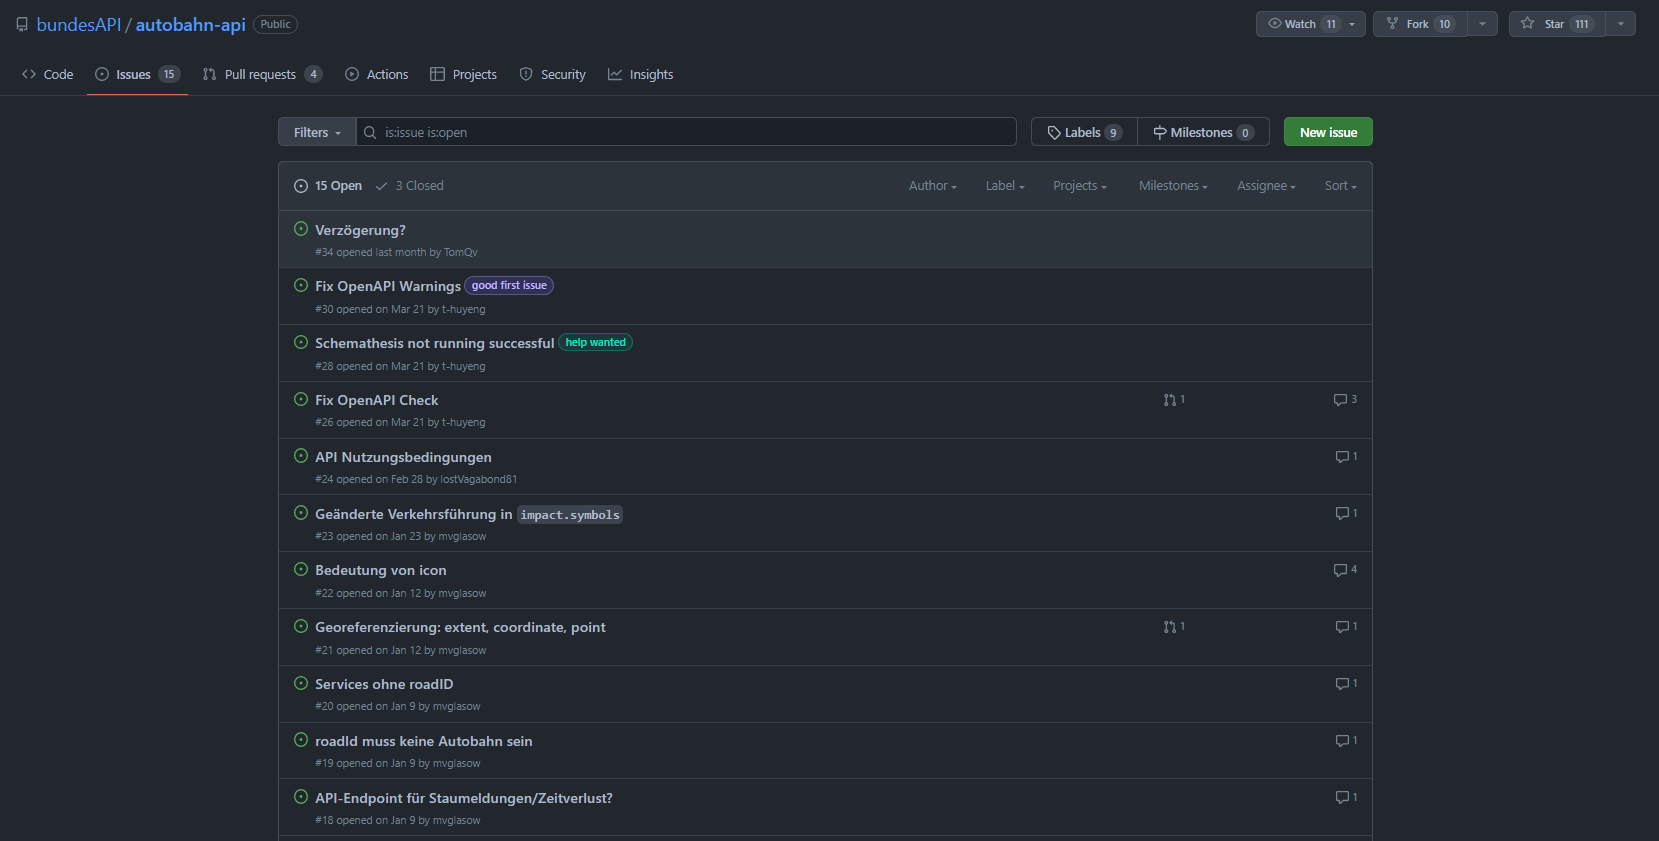
\includegraphics[width=\textwidth]{images/gitissues.png}
  \caption{Gemeldete Probleme}
  \label{fig:gitissues}
\end{figure}

Wie in Abbildung 2 ersichtlich ist, können bei der Erstellung von Problemen verschiedene Tags zugeordnet werden, um eine Klassifizierung für den Entwickler zu erleichtern.
Der Verzeichnisdienst ist ohne vorherige Anmeldung oder Registrierung zugänglich. Ebenso kann der API-Code ohne GIT-Registrierung oder Anmeldung heruntergeladen werden. Das Melden von Problemen über die GIT-Funktion erfordert jedoch eine vorherige Anmeldung und Registrierung. Analog dazu verhält es sich bei verfügbaren Pull Requests und ähnlichen Funktionalitäten.

\subsubsection{Vergleich von API- und datenorientierten Schnittstellen}
REST: protokollorientierte (https://systempilot.net/edi-rest-api-schnittstellen-systemintegration/)
und https://de.wikipedia.org/wiki/Programmierschnittstelle

\begin{tabular}{|L{2cm}|L{2.8cm}|L{2.8cm}|L{2.8cm}|L{2.8cm}|}
\hline
Schnittstellen-Typ & Funktionsorientierte PS & Dateiorientierte PS & Objektorientierte PS & Protokollorientierte PS \\
\hline
Beschreibung & Stellt Funktionen zur Verfügung, die von anderen Anwendungen aufgerufen werden können. & Bietet die Möglichkeit, auf Daten in Dateien zuzugreifen und diese zu verarbeiten. & Basiert auf Objekten, die Funktionen und Eigenschaften enthalten und von anderen Anwendungen verwendet werden können. & Bietet eine strukturierte Art und Weise, um Daten zwischen Systemen auszutauschen. \\
\hline
Beispiele & DLL, Programm-APIs, Bibliotheken & CSV, XML, JSON & COM, CORBA, SOAP & HTTP, TCP/IP, FTP \\
\hline
Verwendung & Häufig in einfachen Anwendungen verwendet. & Nützlich für Anwendungen, die mit großen Datenmengen arbeiten. & Komplexere Anwendungen, die eine umfangreichere Struktur benötigen. & Weit verbreitet in verteilten Systemen und bei der Kommunikation zwischen verschiedenen Anwendungen. \\
\hline
Vorteile & Schnell und einfach zu implementieren. & Gut geeignet für die Arbeit mit großen Datenmengen. & Bietet eine flexible Art der Datenverarbeitung und -speicherung. & Bietet eine standardisierte Art der Kommunikation zwischen Systemen. \\
\hline
Nachteile & Kann bei komplexen Anwendungen unübersichtlich werden. & Begrenzte Funktionalität im Vergleich zu anderen Schnittstellentypen. & Komplex in der Implementierung und erfordert mehr Aufwand. & Kann weniger effizient als andere Schnittstellentypen sein. \\
\hline
\end{tabular}


\subsection{Analyse von Web-APIs}

\subsubsection{Erstellung des Bewertungsmodells}
Erstellen Sie ein Bewertungsmodell für angebotene Web APIs
\begin{itemize}
\item Welche Informationen halten Sie für einen Einsatz notwendig?
\begin{itemize}
\item Spezifikation/Technologie (SOAP, REST, JSON, MIME, …)
\item Servicebeschreibung (technisch \& fachlich)
\item Funktionstüchtigkeit (Qualitätsvereinbarungen)
\item Kontaktinformationen
\item Beispiele zur programmiertechnischen Einbindung
\end{itemize}
\item Informationen zu einem Ansatz für ein Bewertungsmodell – siehe Anlage
\end{itemize}

Wir haben uns dazu entschieden alle API´s aus dem BundDev Verzeichnis zu bewerten. So ist es möglich eine Übersicht der vom Bund bereitgestellten Schnittstellen zu gewinnen. Zu Beginn wurde das Bewertungsmodell in fünf Kategorien aufgeteilt. Diese lauten: Übersicht, Offenheit, Qualität, Dokumentation und Verfügbarkeit.

\begin{enumerate}
\item In diesem Teil wird nur eine Übersicht über die einzelnen API´s dargestellt. Unter welchen URL lässt sich die Dokumentation finden? Wie viele get, post, put, delete und andere werden werden in der API verwendet? Hierbei wird keine Bewertung vorgenommen, sondern es wird nur aufgezählt.
\item Offenheit: 
\begin{itemize}
\item Quellcode: Die Offenlegung des Quellcodes einer API fördert Transparenz und Anpassungsfähigkeit, indem sie Entwicklern Einblicke in die Funktionsweise der API gewährt und die Möglichkeit bietet, die API an individuelle Bedürfnisse anzupassen sowie Fehler zu beheben.
\item Insofern ein Token zur Nutzung notwendig ist, sollte dies einfach, kostenlos und umgehend zur Verfügung gestellt werden (nach Registrierung)
\item Zugänglichkeit: Dokumentation, Beispiele, Kontakt, verwendete Sprache (englisch, keine Fachbegriffe und Abkürzungen) sind nachvollziehbar und gut auffindbar
\item Kontakt: Verantwortlicher und ggfs. Entwickler können direkt erreicht werden
\end{itemize}
\item Qualität: 
\begin{itemize}
\item Granularität: zu gering (wenige Ressourcen mit wenigen Routen geben sehr große Objekte zurück) bis zu hoch (für ``normale'' Usecases müssen für ein clientrelevantes Objekt mehrere Abfragen gestellt werden)
\item TLS: ausschließlich oder Weiterleitung bei HTTP Aufruf (gut) über HTTP möglich (mittel) bis nur unter HTTP erreichbar (schlecht)
\item Statuscode: Werden alle relevanten Statuscodes in den Dokumentationen genannt und ausreichen beschrieben?
\item Ressourcen fachlich korrekt ausgewählt?
\item Routen in angemessener Tiefe?
\end{itemize}
\item Dokumentation:
\begin{itemize}
\item Routen: beschrieben, Datentypen, Beispiele
\item Ressourcen: benannt, Request und Response Modelle verfügbar (required? usw.)
\item Parameter: benannt, Datentypen, Beispiele
\end{itemize}
\item Verfügbarkeit und Performance
\end{enumerate}


\subsubsection{Einsatz des Bewertungsmodells}
Analysieren Sie stichpunktartig 20 registrierte Web APIs
\begin{itemize}
\item Verwenden Sie ihr entwickeltes Bewertungsmodell
\item Ausführung der Services mittels Musterlösung (keine Programmierung)
\end{itemize}
Die zu analysierenden Service-APIs sollten möglichst aus unterschiedlichen Serviceverzeichnissen stammen.

\begin{table}[H]
\begin{center}
\begin{tabular}{|p{3.6cm}|p{8.5cm}|p{2.5cm}|}
\hline
\textbf{Bewertungsteil} & \textbf{Beschreibung} & \textbf{Punkte}\\ \hline
Token/Registrierung & Nicht notwendig ODER notwendig, aber leicht einzurichten. Wenn ja, mit Token sind alle Endpunkte verfügbar & 2\\ \hline
& Notwendig, aber auch dann nicht alle Endpunkte verfügbar ODER notwendig, aber mit Hürden einzurichten & 1\\ \hline
& Für alle Endpunkte nötig UND mit Hürden einzurichten ODER Token ungültig & 0\\ \hline
Quellcode & Liegt vor und ist verlinkt & 1\\ \hline
& Liegt nicht vor oder muss erst gesucht werden & 0\\ \hline
Request Limit & Wenn nicht angegeben, stellen wir verteilt über 30 Minuten 1000 Anfragen. Wenn das klappt, gibt es zwei Punkte. & \\ \hline
& $<$ 100 & 0 \\ \hline
& $<$ 1000 & 1 \\ \hline
& $<$ 10k & 2 \\ \hline
& $>$ 10k & 3 \\ \hline
Kontakt & Ja (Link/E-Mail) & 1 \\ \hline
& nein & 0 \\ \hline
\end{tabular}
\caption{Bewertungsschema Offenheit}
\label{Offenheit}
\end{center}
\end{table}

\begin{table}[H]
\begin{center}
\begin{tabular}{|p{3.6cm}|p{8.5cm}|p{2.5cm}|}
\hline
\textbf{Bewertungsteil} & \textbf{Beschreibung} & \textbf{Punkte}\\ \hline
Granularität & Ausgeglichen, sowohl Listen als auch Einschränkungen auf einzelne Objekte & 1 \\ \hline
& Sehr viele Use Cases mit einzelnen Endpunkten oder eine Anfrage erfordert verschiedene Ressourcen & 0 \\ \hline
& Zu geringe Granularität, sehr wenige Endpunkte mit zu umfangreichen Datenmodellen & 0 \\ \hline
Transportverschlüsselung & HTTPS und gegebenenfalls Weiterleitung von HTTP auf HTTPS & 2 \\ \hline
& HTTP und HTTPS, aber keine Weiterleitung von HTTP & 1 \\ \hline
& Nur HTTP & 0 \\ \hline
Routen & Jede Ressource hat einen Identifier und ist mit Nomen benannt. HTTP-Methoden sind korrekt eingesetzt. Maximale Tiefe beträgt 3. & 2 \\ \hline
& Mindestens 2 Bedingungen aus 2 sind erfüllt & 1 \\ \hline
& Eine oder keine Bedingung aus 2 erfüllt & 0 \\ \hline
Statuscodes & 200, 201, 204, 400, 401, 403, 404, 409, 500, 503 & 2\\ \hline
& Mind. 200, 201, 400, 404, 500 & 1\\ \hline
& Keine & 0\\ \hline
MIME Types & JSON und/ oder XML/ plain text & 2\\ \hline
& Nur XML und/ oder plain text & 1\\ \hline
& Keine/ plain & 0\\ \hline
Versionierung & Verschiedene Majorversionen = 2 & \\ \hline
& Nur latest = 1 & \\ \hline
& Nicht angegeben = 0 & \\ \hline
\end{tabular}
\caption{Bewertungsschema Qualität}
\label{quality}
\end{center}
\end{table}


\begin{table}[H]
\begin{center}
\begin{tabular}{|p{3.6cm}|p{8.5cm}|p{2.5cm}|}
\hline
\textbf{Bewertungsteil} & \textbf{Beschreibung} & \textbf{Punkte}\\ \hline
Routen & alle Routen mit Beispielen (Request/Response), wenn nicht sprechend mit Erläuterung, alle notwendigen und optionalen Parameter sind angegeben & 2 \\ \hline
& wie zwei, aber nur teilweise erfüllt & 1 \\ \hline
& Keine Doku & 0 \\ \hline
Ressourcen & alle Resourcen dokumentiert mit Beispielen, Datentyp und ggfs. default Wert & 2 \\ \hline
& wie zwei, aber nur teilweise erfüllt & 1 \\ \hline
& Keine Doku & 0 \\ \hline
Parameter & alle Parameter mit Datentyp, erlaubtem Werteraum, required und - wenn nicht sprechend - mit Beispiel, ggfs Differenzierung der Rückgabeobjekte ist dokumentiert & 2 \\ \hline
& wie zwei, aber nur teilweise erfüllt & 1 \\ \hline
& Keine Doku & 0 \\ \hline
Statuscodes & Responsecodes mit Zahl, Rückgabestring und Datentyp, Mimetype oder Datenmodell dokumentiert & 2 \\ \hline
& wie zwei, aber nur teilweise erfüllt & 1 \\ \hline
& Keine Doku & 0 \\ \hline
Swagger & Swagger yaml oder json file vorhanden, sowie Swagger UI zum ausprobieren, alle Beispiele und ggfs Auth./Tokens in Swagger UI funktionieren & 2 \\ \hline
& Swagger yaml file oder json vorhanden, aber keine Swagger UI oder andere Möglichkeit zum ausprobieren & 1 \\ \hline
& Keine Doku/ Möglichkeit zum Testen & 0 \\ \hline
\end{tabular}
\caption{Bewertungsschema Dokumentation}
\label{documentation}
\end{center}
\end{table}

\subsection{API - Spezifikationen}
\subsubsection{Spezifikationsanalyse}
Analysieren Sie Struktur und Elemente einer WSDL, OpenAPI-(Swagger) oder auch GraphQL(Schema)-Spezifikation.
\begin{itemize}
\item Verwenden Sie zur Analyse 5 ausgewählte Services
\item Stichpunktartige Beschreibung der Struktur/Unterelemente
\item Metrische Erfassung der Struktur bzw. eingesetzten Elemente
\item Statistische Auswertung Informationen (z.B. Tabellen, Diagramme)
\end{itemize}

\subsubsection{Analysetools}
Nutzen Sie ggf. verfügbare Hilfsmittel und gehen Sie auf die entsprechende Funktionsweise der Tools ein
\begin{itemize}
\item Beispiele: soapUI, SOAPSonar, Postman https://www.postman.com
\item Grafische WSDL-Editoren (z.B. XMLSpy ab Version 8)
\end{itemize}

\subsubsection{Einschränkungen und Alternativen}
\begin{itemize}
\item Welche Informationen fehlen bei der gewählten Spezifikationen?
\item Recherchieren Sie nach alternativen Beschreibungsformen?
\end{itemize}


\newpage
\section{Übung 3b: Entwicklung eigener Service-Angebote}
\subsection{Möglichkeiten für Implementierung und Deployment}
\subsubsection{Analyse der Möglichkeiten}
Analysieren Sie mit Hilfe des Internets mögliche Alternativen zur Implementierung und Deployment von Web APIs (speziell WSDL/XML, REST/OpenAPI und GraphQL), wie z.B.:
\begin{itemize}
\item IDE NetBeans und GlassFish Server
\item IDE Eclipse und Tomcat \& Axis-Erweiterung
\item Postman API Builder
\item Cloud-basierte Entwicklung/Deployment
\end{itemize}

Nach weitreichender Internetrecherche wurden einige Werkzeuge zur Implementierung und Deployment von Apis zusammengetragen. Zur besseren Einordnung dieser sind Eigenschaften wie Scope und Typ sowie falls vorhanden Laufzeitanforderungen aufgeführt. 

\begin{table}[h]
\centering
\begin{tabular}{|L{4cm}|L{3cm}|L{2cm}|L{2cm}|}
\hline
\textbf{Plattform / Service} & \textbf{Scope} & \textbf{Typ} & \textbf{Laufzeit} \\ \hline
AWS Lamda mit AWS API Gateway & Implementierung, Deployment & SaaS & - \\ \hline
ApiGee & Implementierung, Deployment & SaaS & - \\ \hline
Postman Api Builder & Implementierung & SaaS & - \\ \hline
Firebase & Implementierung, Deployment & SaaS & - \\ \hline
Swagger Hub & Deployment & SaaS & - \\ \hline
Cloudflare Workers & Deployment & FaaS & - \\ \hline
Supabase & Implementierung, Deployment & PaaS & - \\ \hline
AWS Amplify & Deployment & PaaS & - \\ \hline
AWS ECS & Deployment & IaaS & - \\ \hline
Swagger Codegen & Implementierung & Executable & Java \\ \hline
Apicurio Studio & Implementierung & Executable & Java \\ \hline
ASP.NET & Implementierung & Framework & C\# \\ \hline
express.js & Implementierung & Framework & JS \\ \hline
Flask & Implementierung & Framework & Python \\ \hline
Spring Boot & Implementierung & Framework & Java \\ \hline
Ruby on Rails & Implementierung & Framework & Ruby \\ \hline
\end{tabular}
\caption{Übersicht über verschiedene Plattformen und Services für die Implementierung, Deployment und Nutzung von APIs.}
\label{api-platforms}
\end{table}


\subsubsection{Analytischer Vergleich der Möglichkeiten}
Vergleichen Sie die gefunden Alternativen anhand eines eigenen Bewertungsmodells, mit Hilfe von Kriterien wie z.B.:
\begin{itemize}
\item Voraussetzungen zur Verwendung (HW- und SW-Ressourcen)
\item Integration von Entwicklung- und Ausführungsplattform
\item DevOps orientierte Vorgehensweise (Automationsaspekte)
\item Verbreitung, Entwicklersupport, Kosten, Lizenzen
\end{itemize}

Im Folgenden werden ausgewählte der in 3b.1.1 aufgeführten Implementierungs- und Deploymentmöglichkeiten mittels eines Bewertungsschemas verglichen. Die ausgewählten tools stehen exemplarisch für jeweils eine Implementierungs- oder Deploymentart.

\paragraph{Implementierung} \mbox{} \\
Das der Bewertung verschiedener Implementierungsarten zugehörige Schema beinhaltet die Kriterien Komplexität der Implementierung, Komplexität der OpenApi-Spezifikationserstellung, Güte der Dokumentation, Popularität, Kosten und Geschwindigkeit. Zur Bewertung der Implementierungskomplexität werden die Implementierungen der gleichen Api verglichen. Dazu wird die künstliche Intelligenz ChatGPT genutzt. Diese bekommt pro Implementierungsart die gleiche Aufforderung, welche wie folgt aussieht: 
\begin{formal}
Implement a rest api with one endpoint named /items. This endpoint should return all columns of the mysql database table item and should be able to response the http-codes 200, 404 and 500. Do so using the shortest possible way in {Implementierungsart}.
\end{formal}

Die Ergebnisse wurden dann auf die Herkunft der nötigen libraries sowie die Anzahl der Funktionaufrufe untersucht. Zur Bewertung der Komplexität der OpenApi Spezifikationserstellung wurde recherchiert, ob eine Spezifikationserstellung überhaupt möglich und wenn möglich ohne externe Hilfsmittel/Libraries möglich ist. Außerdem wurde berücksichtigt, ob die Erstellung automatisch oder manuell erfolgt. Zur effektiven Entwicklung von Software sind umfangreiche, verständliche und vor allem aktuelle Dokumentationen von großer Bedeutung. Aufgrund dessen ist auch die Dokumentationsgüte teil des Bewertungsschemas. Hier fließen die Übersichtlichkeit, der Umfang, die Aktualität und die Verständlichkeit ein. Dabei gilt zu beachten, dass diese Bewertungen nicht objektiv messbar sind und daher subjektiv bewertet wurden. Außerdem wurde die Popularität mittels Google Trends bestimmt. Die Geschwindigkeit wurde anhand von Benchmarks gerankt. Ein weiteres sehr wichtiges Kriterium zu Auswahl der Entwicklungswerkzeuge ist die Preisstruktur dieser, weshalb diese ebenfalls aufgeführt ist.

\begin{lstlisting}[language=Java,frame=single,caption=Implementierung in Java,label=toml]
import java.sql.ResultSet;
import java.sql.SQLException;
import java.util.List;

import org.springframework.beans.factory.annotation.Autowired;
import org.springframework.http.HttpStatus;
import org.springframework.http.ResponseEntity;
import org.springframework.jdbc.core.JdbcTemplate;
import org.springframework.jdbc.core.RowMapper;
import org.springframework.web.bind.annotation.GetMapping;
import org.springframework.web.bind.annotation.RequestMapping;
import org.springframework.web.bind.annotation.RestController;

@RestController
@RequestMapping("/items")
public class ItemController {

    public static void main(String[] args) {
        SpringApplication.run(Main.class, args); 
    }

    @Autowired
    private JdbcTemplate jdbcTemplate;

    @GetMapping
    public ResponseEntity<List<Item>> getAllItems() {
        try {
            List<Item> items = jdbcTemplate.query(
                    "SELECT * FROM item",
                    new RowMapper<Item>() {
                        public Item mapRow(ResultSet rs, int rowNum) throws SQLException {
                            Item item = new Item();
                            item.setId(rs.getLong("id"));
                            item.setName(rs.getString("name"));
                            item.setDescription(rs.getString("description"));
                            item.setPrice(rs.getDouble("price"));
                            return item;
                        }
                    });
            if (items.isEmpty()) {
                return new ResponseEntity<>(HttpStatus.NOT_FOUND);
            }
            return new ResponseEntity<>(items, HttpStatus.OK);
        } catch (Exception e) {
            return new ResponseEntity<>(null, HttpStatus.INTERNAL_SERVER_ERROR);
        }
    }

    public static class Item {
        private long id;
        private String name;
        private String description;
        private double price;

        public long getId() {
            return id;
        }

        public void setId(long id) {
            this.id = id;
        }

        public String getName() {
            return name;
        }

        public void setName(String name) {
            this.name = name;
        }

        public String getDescription() {
            return description;
        }

        public void setDescription(String description) {
            this.description = description;
        }

        public double getPrice() {
            return price;
        }

        public void setPrice(double price) {
            this.price = price;
        }
    }
}

\end{lstlisting}

\begin{lstlisting}[language=Python,frame=single,caption=Implementierung in python,label=toml]
from flask import Flask, jsonify
from flask_mysqldb import MySQL

app = Flask(__name__)
app.config['MYSQL_HOST'] = 'localhost'
app.config['MYSQL_USER'] = 'username'
app.config['MYSQL_PASSWORD'] = 'password'
app.config['MYSQL_DB'] = 'database'
mysql = MySQL(app)

@app.route('/items')
def get_items():
    cur = mysql.connection.cursor()
    cur.execute("SELECT * FROM item")
    data = cur.fetchall()
    if data:
        return jsonify(data), 200
    else:
        return jsonify({"message": "No items found"}), 404

@app.errorhandler(500)
def internal_error(error):
    return jsonify({"message": "Internal server error"}), 500

if __name__ == '__main__':
    app.run(debug=True)
\end{lstlisting}

\begin{lstlisting}[language=Java,frame=single,caption=Implementierung in C\#,label=toml]
using Microsoft.AspNetCore.Builder;
using Microsoft.AspNetCore.Http;
using Microsoft.Extensions.DependencyInjection;
using Dapper;
using MySql.Data.MySqlClient;
using System;
using System.Linq;

var builder = WebApplication.CreateBuilder(args);

builder.Services.AddSingleton<MySqlConnection>(sp =>
    new MySqlConnection(builder.Configuration.GetConnectionString("DefaultConnection")));

var app = builder.Build();

app.MapGet("/items", async (HttpContext httpContext, MySqlConnection connection) =>
{
    try
    {
        var items = (await connection.QueryAsync<Item>("SELECT * FROM Items")).ToList();
        if (items.Count == 0)
        {
            return Results.NotFound();
        }
        return Results.Ok(items);
    }
    catch (Exception ex)
    {
        Console.Error.WriteLine(ex);
        return Results.StatusCode(StatusCodes.Status500InternalServerError);
    }
});

app.Run();

public record Item(int Id, string Name, string Description, decimal Price, DateTime CreatedAt);
\end{lstlisting}

\begin{table}[H]
  \centering
  \caption{Bewertungskriterien für API-Testtools}
    \begin{tabular}{|L{2.5cm}|L{3cm}|L{5.5cm}|L{3cm}|}
    \hline
    Kriterium & Unterkategorie & Bewertungen & Quellen \\
    \hline
    Komplexität der Implementierung & notwendige Hilfsmittel/Libraries & 1: keine externen Hilfsmittel/Libraries nötig \newline 0: externe Hilfsmittel/Libraries nötig &  \\
\cline{2-4}          & Anzahl der notwendigen Schritte/Funktionsaufrufe & 0: mehr als der Durchschnitt der anderen \newline 1: durchschnittlich \newline 2: weniger als der Durchschnitt der anderen &  \\
    \hline
    OpenAPI-Spezifikation & Integration & 2: out of the box \newline 1: Drittanbieter library \newline 0: nicht möglich & Spring: \footnote{https://spring.io/} \newline Flask: \footnote{https://flask.palletsprojects.com/en/2.1.x/} \newline .NET: \footnote{https://dotnet.microsoft.com/} \newline Postman: \footnote{https://www.postman.com/} \\
    \hline
    Implementierung & & 2: automatisch \newline 1: manuell &  \\
    \hline
    Dokumentation & Übersichtlichkeit (logische Untergliederung) & 1: übersichtlich \newline 0: unübersichtlich & Spring: \footnote{https://spring.io/} \newline Flask: \footnote{https://flask.palletsprojects.com/en/2.1.x/} \newline .NET: \footnote{https://dotnet.microsoft.com/} \newline Postman: \footnote{https://www.postman.com/} \\
    \hline
    Umfang & & 1: vollumfänglich \newline 0: unvollständig &  \\
    \hline
    Aktualität & & 1: aktuell \newline 0: (teils) veraltet &  \\
    \hline
    Verständnis (ggf. mit Beispielen) & & 1: gut verständlich \newline 0: nicht gut verständlich &  \\
    \hline
    Popularität & - & Rangfolge entsprechend Google Trends (0-3) & \footnote{https://trends.google.com/trends/explore?q=swagger\%20ui,postman,insomnia\&geo=US} \\
    \hline
    Geschwindigkeit & - & Rangfolge entsprechend TechEmpower Benchmark (0-2) & \footnote{https://www.techempower.com/benchmarks/} \\
    \hline
    \end{tabular}%
  \label{tab:bewertungskriterien}%
\end{table}%


\paragraph{Deployment} \mbox{} \\
Ähnlich dem Vergleich der Implementierungsmöglichkeiten wurden auch für den Deploymentmöglichkeiten-Vergleich repräsentative Vertreter für die drei verbreitetsten Arten Application Server, Cloud Server und Container gewählt. Diese wurden bezüglich der Skalierbarkeit und der Continuous-Deployment-Fähigkeit verglichen. Dabei wurde zur Bewertung der Skalierbarkeit die Replizierbarkeit und das Möglichkeit von Loadbalancing sowie die Effizienz herangezugen um so die Fähigkeit zum vertikalem Skalieren abzubilden. Die Continuous Deployment Fähigkeit wird damit bestimmt, ob dies grundsätzlich möglich ist und wenn ja, mit oder ohne Server Downtime. \\

\begin{tabular}{|L{2cm}|L{3.2cm}|L{1.5cm}|L{1.5cm}|L{1.5cm}|L{1.5cm}|L{1.5cm}|}
\hline
& Kriterium & Aws Api Gateway & Azure Api Management & Linode & AWS EC2 & On Premise \\ \hline
Flexibilität Entwicklung & mehrere Sprachen & + & + & + & + & + \\ 
& vorgegebene Libraries/Frameworks & + & + & + & + & + \\ 
& Api-Dokumentaion/-Spezifikation & + & + & + & + & + \\ \hline
Flexibilität Deployment & Integration in CD Pipelines & / & + & + & + & + \\ 
& Restriktionen & ? & ? & + & + & + \\ 
& verschiedene Umgebungen (Test/Production) & + & + & + & + & + \\ 
& parallele Versionen möglich & + & + & + & + & + \\ \hline
Skalierbarkeit & Containerisierung möglich & ? & + & / & / & / \\ 
Kosten & initial & + & + & + & + & - \\ 
& laufend & - & - & / & / & / \\ \hline
Abhängigkeiten & vorgeschriebene Libraries/Frameworks & + & + & + & + & + \\ 
& Abhängigkeit von Anbieter selbst & - & - & - & - & + \\ 
& Laufzeitumgebung & / & / & - & / & + \\ \hline
\end{tabular}

\subsection{Entwicklung}
\subsubsection{Rahmenbedingungen}
Wählen Sie für die weiteren Aufgaben dieser Übung eine konkrete Entwicklungsumgebung aus, begründen Sie Ihre Entscheidung
\begin{itemize}
\item Benötigte Softwareversionen und Werkzeuge
\item Installation und Konfiguration der Entwicklungsumgebung
\item Cloud-basierte Implementierung und Betrieb
\end{itemize}
 
 Für eine nachvollziehbare Argumentation, warum der eingesetzte Toolstack verwendet wurde und welche Laufzeitumgebung und Art des Deployments als angebracht eingeschätzt wurde, sollen zunächst kurz die Anforderungen an die Anwendung dargestellt werden. Diese sind zwar ``simuliert'', jedoch (in sehr oberflächlicher Form) an möglichen realen Anforderungen angelehnt. Da die nicht-funktionalen Anforderungen hier eher die Argumentationsgrundlage bilden, stehen diese im Fokus - funktionale Anforderungen sollten nur in Ausnahmefällen eine Determinante für Techstack und Deployment sein.  \\
Überlegungen, welche eine prototypische Umsetzung im gegebenen Rahmen sprengen würden, werden bewusst außer acht gelassen. Dazu gehören: ggfs. initial höhere Entwicklungskosten, verfügbare (Entwicklungs)ressourcen und Skillset der Beteiligten, architektonische Überlegungen und der Einsatz bestimmter Design Patterns, sowie das Thema Tests. \\
Desweiteren halten wir eine Begründung, warum nun welche Entwicklungsumgebung eingesetzt wurde, nicht für sinnvoll. Welche IDE ein Entwickler verwendet, ob als Git nun Github, Gitlab oder Bitbucket verwendet wird und mit welchem Tool REST Endpunkte getestet werden ist entweder von den Vorlieben und Gewohnheiten des Einzelnen abhängig, oder durch Vorgaben des Arbeitgebers bestimmt (oder beides). Insofern beschränken wir uns bei diesen Punkten auf die Benennung der ``Werkzeuge'', ohne das Warum weiter zu vertiefen. Stattdessen wollen wir die aus unserer Sicht viel wichtigere Frage beantworten, warum für den genannten Usecase eine bestimmte Sprache, Bibliotheken und Deploymentszenarien gewählt wurden.
 
\paragraph{Anforderungen} \mbox{} \\

Funktionale Anforderungen:
\begin{itemize}
\item Anzeige von Basisinformationen zu Coderepositories (Autor, Sprache, Forks, Commits), welche über eine REST API abgerufen werden
\item Löschen vorhandener, Hinzufügen neuer und Ändern vorhandener Repositories (Client)
\item Persistierung der Änderungen in einer Datenbank
\item Bereitstellung als Webapp
\end{itemize}

Nicht-funktionale Anforderungen: 
\begin{itemize}
\item unterdurchschnittlich geringe TCO durch:
\begin{itemize}
\item hohe Performanz und geringen Footprint bei der Hardwarenutzung
\item geringe Wartungskosten
\item einfache Verwaltung der Abhängigkeiten
\item einfaches Deployment
\end{itemize}
\item gute Skalierbarkeit
\item hohes Level an Sicherheit
\item volle Flexibilität hinsichtlich der Laufzeitumgebung
\item DB Typ möglichst offen
\end{itemize}



\paragraph{Verwendete Sprache(n)} \mbox{} \\

Client und REST API sollen in Rust geschrieben werden, auch die verwendete Datenbank (Surreal DB) ist in Rust geschrieben. Rust ist eine multi-paradigmatische, noch recht junge (2015) Programmiersprache, die auf konzeptioneller Ebene einige Besonderheiten aufweist. Im Folgenden werden einige dieser Besonderheiten erläutert:
\begin{itemize}
\item Memory-Safety und Thread-Safety: Rust erreicht dies durch eine strenge Typisierung und durch Speicherzugriffsregeln, die sicherstellen, dass Speicher nur dann gelesen oder geschrieben werden kann, wenn es korrekt und sicher ist. Dies wird durch die Borrowing- und Ownership-Konzepte erreicht, die den Zugriff auf den Speicher in Rust stark reglementieren. Mit diesen Regeln ist es möglich, Memory-Safety-Garantien zu erzwingen, ohne dass ein Garbage-Collector erforderlich ist, aber auch ohne den in C und C++ verwendeten Ansatz der manuellen Speicherkontrolle.
\item Laufzeitstabilität: Rust ist dafür bekannt, Laufzeitfehler quasi auszuschließen (von daher der Name - einmal ausgerollt kann die Anwendung vor ich hin rosten). Dies wird durch eine Kombination aus verschiedenen Techniken erreicht, darunter die bereits erwähnten Konzepte, den Verzicht auf nulls und einen in vielen Fällen funktionalen Programmierstil. Ausschlaggebend für die hohe Laufzeitstabilität ist zudem der tiefgreifende Compiler, der bereits bei der Übersetzung des Codes umfangreiche Fehlerprüfungen durchführt. Dadurch werden viele potenzielle Fehlerquellen bereits im Vorfeld erkannt und beseitigt.
\item Gute Dokumentation: Die Gesamtdokumentation, insbesondere das Rust Book, aber auch die Dokumentation der einzelnen Bibliotheken, bietet sowohl Einsteigern als auch erfahrenen Entwicklern Hilfestellungen, um die Sprache zu erlernen und ihre Fähigkeiten zu verbessern.
\item Management von Abhängigkeiten: das Management von Abhängigkeiten durch das Cargo-Build-System garantiert eine Kompatibilität der (transitiven) Abhängigkeiten und ein replizierbares Kompilat/Binary, sowie durch SemVer eine einfache Verwaltung der Abhängigkeiten
\item Rust hat eine schnell wachsende Community und wird von immer mehr Unternehmen für die (Re)implementierung kritischer Komponenten eingesetzt (z.B. npm, Cloudflare und AWS Lambda). Teile des Android Kernels, sowie des Linuxkernels und neuerdings auch Systemkomponenten in Windows werden in Rust neu geschrieben. Diese Entwicklung deutet auf eine stabile Zukunft sowohl hinsichtlich technischem Support, also auch wachsender Entwicklerressourcen hin - ein gewichtiges Argument bei der Businessentscheidung für eine Sprache.
\end{itemize}

\paragraph{Komponenten} \mbox{} \\
Aus der Beschreibung in Verbindung mit den nicht funktionalen Anforderungen lässt sich die Entscheidung für Rust für die systemkritischen (REST API) Komponenten ableiten. Sicherheit, Stabilität, eine hohe Flexibilität der Laufzeitumgebungen, Performanz (s. auch Abb.\ref{fig:apibenchmark} sowie voraussichtlich geringe TOC sind bei einer Umsetzung mit Rust wahrscheinlicher als in den meisten anderen Sprachen. Microsoft führt beispielsweise einen großen Teil der Schwachstellen auf fehlerhafte Speicherverwaltung zurück, dieses Risiko wird durch die garantierte Memory-Safety minimiert:
\begin{formal}
``Microsoft revealed at a conference in 2019 that from 2006 to 2018 70 percent of their vulnerabilities were due to memory safety issues. Google also found a similar percentage of memory safety vulnerabilities over several years in Chrome.''\footnote{https://media.defense.gov/2022/Nov/10/2003112742/-1/-1/0/CSI\_SOFTWARE\_MEMORY\_SAFETY.PDF}
\end{formal}


\begin{figure}[H]
\centering
  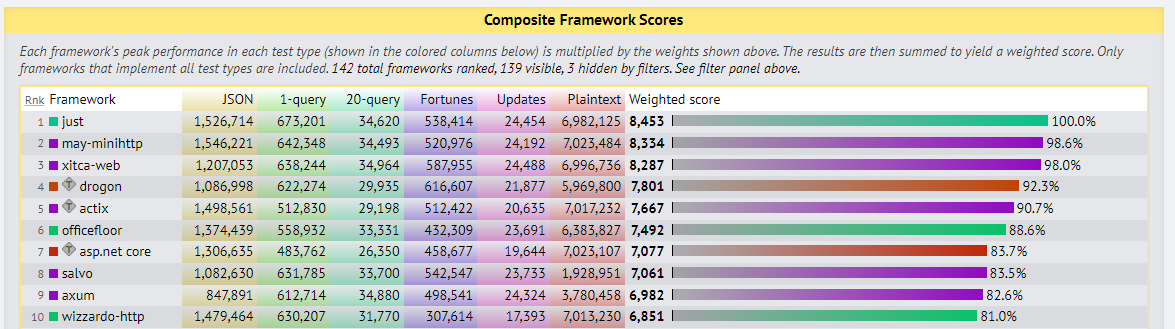
\includegraphics[width=\textwidth]{images/score3.png}
  \caption{Benchmark Backend Webframeworks}
  \label{fig:apibenchmark}
\end{figure}


Die Entscheidung auch das Frontend in Rust zu implementieren war hingegen eher experimenteller Natur und würde - auch aufgrund der teils noch nicht ausgereiften Frameworks - in einer realen Situation vermutlich anders ausfallen. Dennoch soll die Entscheidung an dieser Stelle kurz begründet werden. \\

Da Rust problemlos in Maschinencode als auch Webassembly (Entwicklung 2018) kompiliert werden kann, verzichten die meisten Webframeworks, die in Rust geschrieben sind, komplett auf Javascript. Systemnahe Sprachen, typischerweise Assembler, C++ oder Rust, aber auch interpretierte Sprachen wie C\# können mit der Laufzeitumgebung Webassembly in bytecode kompiliert werden, welcher plattformunabhängig und extrem schnell im Browser, zunehmend aber auch auf verteilten Systemen ausgeführt wird. Da die Last durch die Ausführung der Anwendungslogik im Browser hier auf Clientseite liegt, impliziert der Ansatz ein Abrücken vom traditionellen Client-Server Paradigma. Das verwendete Framework Dioxus zeichnet sich durch seinen Reactive Ansatz (ähnlich Svelte oder Solid.js), sowie eine sehr hohe Performanz aus (s. auch Abb.\ref{fig:clientbenchmark}. Zudem ist auch das Deployment für Mobiles und Desktoplattformen möglich.

\begin{figure}[H]
\centering
  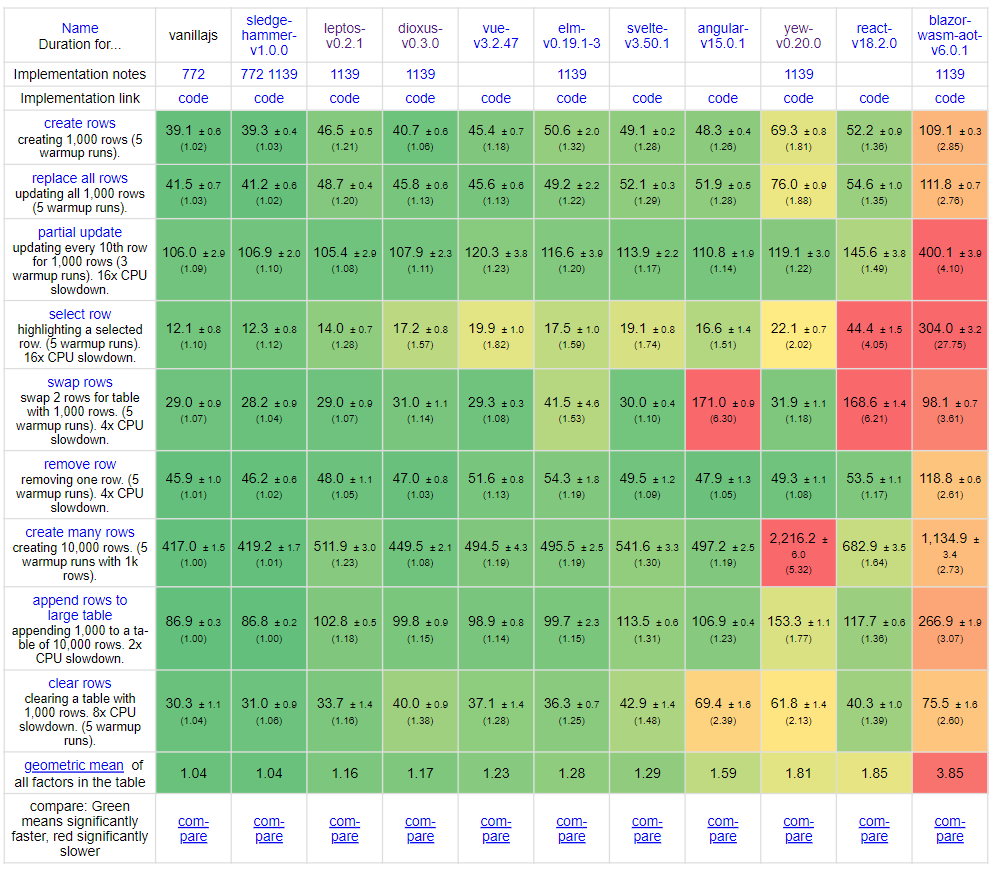
\includegraphics[width=\textwidth]{images/bm.png}
  \caption{Benchmark Frontend Webframeworks}
  \label{fig:clientbenchmark}
\end{figure}


DB

\paragraph{Eingesetzte Frameworks und Libraries} \mbox{} \\

\begin{table}[H]
\begin{center}
\begin{tabular}{| L{2cm} | L{2cm} | L{3.2cm} | L{3.2cm} | L{3.2cm} |}
\hline
Service- komponente & Name (Version) & Funktion & Vorteil & Nachteil \\ \hline
Client & Sycamore & Webassembly Webframework & & \\ \hline
Client & Perseus & Sycamore Erweiterung & & \\ \hline
REST API & Serde & JSON (De)serialisierung & & \\ \hline
REST API & Actix & Webserver & & \\ \hline
REST API & utoipa & Open API Doc Generation & & \\ \hline
Datenbank & Surreal DB & vollständiges DBMS und integrierter Server & & \\ \hline 
\end{tabular}
\caption{Verwendete, externe Abhängigkeiten}
\label{dependencies}
\end{center}
\end{table}


\begin{lstlisting}[language=SQL,frame=single,caption=cargo.toml Datei zur Organisation der Abhängigkeiten in Rust,label=toml]
[package]
name = "rust-actix-surreal-rest-api"
version = "0.1.0"
edition = "2021"
authors = ["Hannes Roever"]

[dependencies]
actix-web = "4"
actix-cors = "*"
serde = {version = "1.0.152", features = ["derive"]}
serde_json = {version = "1.0.93"}
tokio = { version = "1", features = ["full"] }
mini-redis = "0.4"
env_logger = "0.10.0"
log = "0.4"
futures = "0.3"
utoipa = { features = ["actix_extras"] }
utoipa-swagger-ui = { features = ["actix-web"] }
chrono = "*"
reqwest = {features = ["json"]}
\end{lstlisting}

\paragraph{Konfiguration Entwicklungsumgebung} \mbox{} \\
Voraussetzung für die dargestellten Schritte ist, dass Docker bereits installiert ist (Docker Client auf Windows, Docker Engine auf Linux). Da dies, analog zum Vorhandensein einer geeigneten IDE oder eines Editors, zu den Basiswerkzeugen in der Entwicklung gehört, wird der allgemeine Installations- und Konfigurationsprozess nicht weiter ausgeführt (zumal er sich je nach OS auch unterscheidet und bestens dokumentiert ist).

\subparagraph{Datenbank} \mbox{} \\
Die Datenbank kann sehr unkompliziert als Docker-Container gestartet werden. Das entsprechende CLI Kommando bzw. der Inhalt und das Kommando zum Ausführen der docker-compose.yml sind in den Listings \ref{surrealdockerone}-\ref{surrealdockerthree} dargestellt. s sollte nur eine der Optionen genutzt werden. Anschließend läuft die Datenbank mit in-memory Option (weitere sind möglich) unter Port 8000 des localhost.

\begin{lstlisting}[language=SQL,frame=single,caption=CLI Command zum Starten des Datenbankcontainers,label=surrealdockerone]
docker run --rm --pull always -p 8000:8000 surrealdb/surrealdb:latest start
\end{lstlisting}

\begin{lstlisting}[language=SQL,frame=single,caption=Alternative mit docker-compose zum Starten des Datenbankcontainers,label=surrealdockertwo]
version: '3.8'
services:
  db:
    image: surrealdb/surrealdb:latest
    restart: always
    command: start --user root --pass root memory
    ports:
      - '8000:8000'
    volumes: 
      - db:/var/lib/surrealdb/data
volumes:
  db:
    driver: local
\end{lstlisting}

\begin{lstlisting}[language=bash,frame=single,caption=CLI Command zum Ausführen der docker-compose Datei. Das Kommando muss im Verzeichnis ausgeführt werden\, in dem die Datei liegt\, oder der Pfad der Datei über die flag --f spezifiziert werden,label=surrealdockerthree]
docker-compose up -d
\end{lstlisting}

\subparagraph{REST API} \mbox{} \\
Für die Entwicklung in Rust wird die Rust Toolchain benötigt (bestehend aus rustup, rustc und cargo). Die Installation erfolgt über die Kommandozeile oder für Windows mit einem Installer, welcher unter https://www.rust-lang.org/tools/install heruntergeladen werden kann. Ggfs. muss noch die ensprechende Umgebungsvariable gesetzt werden. Die Toolchain umfasst alle notwendigen Commandlinetools für die Kompilierung, Codeformatierung, Abruf von Dokumentation (ähnlich zu MAN Pages), Tests und Deployment. 

\begin{lstlisting}[language=bash,frame=single,caption=CLI Command zur Installation von Rust in Linux und macOS,label=rustinstallationone]
curl --proto '=https' --tlsv1.3 https://sh.rustup.rs -sSf | sh
\end{lstlisting}

Für die Erstellung eines neuen Projekts muss das Kommando cargo new projektname ausgeführt werden. Im entsprechenden Verzeichnis wird ein Ordner mit den Konfigfiles, main und Gitrepository angelegt. Die Bearbeitung des Codes kann mit einem einfachen Editor (z.B. Vim, Neovim, Emacs, Sublime, Nano), einem erweiterten Editor (VS Code) oder einer vollumfänglichen IDE (Intellij IDEA, CLion) vorgenommen werden. Wir nutzen IntelliJ und für die schnelle Bearbeitung, z.B. auf einem über SSH verbundenen Server, Nano. \\
Weitere Schritte sind nicht notwendig, die Abhängigkeiten können in der cargo.toml (s.a. Listing \ref{toml}) Datei hinzugefügt werden und werden beim nächsten Build, so noch nicht lokal vorhanden, automatisch gezogen und kompiliert. Mit cargo run (bauen, ausführen) bzw cargo build (bauen), fürs publishing mit --release flag, wird das Programm ausgeführt. 

\subparagraph{Client WebApp} \mbox{} \\
Um die Kompilierung in WASM zu ermöglichen sind zwei weitere, global bereitzustellende Abhängigkeiten notwendig, die Installation ist in Listing \ref{rustinstallationtwo} zu sehen.

\begin{lstlisting}[language=bash,frame=single,caption=CLI Command zur Installation der Laufzeitumgebung webassembly und des WASM-Buildtools Trunk für Rust,label=rustinstallationtwo]
rustup target add wasm32-unknown-unknown
cargo install --locked trunk
\end{lstlisting}

Der Start eines bereits erstellten Projektes kann mit trunk --serve durchgeführt werden, durch das Buildtool wird automatisch ein lokaler Webserver bereitgestellt. Perseus baut auf Sycamore auf und kann mit den Commands aus Listing \ref{perseusone} installiert und ausgeführt werden.

\begin{lstlisting}[language=bash,frame=single,caption=CLI Command zur Installation der Perseus CLI und Ausführung eines Projektes,label=perseusone]
cargo install perseus-cli
perseus serve -w
\end{lstlisting}

\paragraph{Deployment} \mbox{} \\
Das Deployment wird, dem Industriestandard folgend, als Containerlösung realisiert. Um den Rahmen nicht zu sprengen, haben wir uns für Docker entschieden und auf einen Orchestrierungslayer, z.B. mit K8, verzichtet. Die physische Bereitstellung erfolgt bei einem IAAS Anbieter, aufgrund der Nutzung von Docker ist die Linux-Distribution zweitrangig - Debian oder Ubuntu als etablierte Serverdistros oder Alpine als Low-Footprint Distro sind naheliegende Optionen. Windows Server oder spezielle oder proprietäre Lösungen sind nicht notwendig und u.E. auch nicht sinnvoll, weil sie eine Abhängigkeit von einer bestimmten Firma bzw. Technologie schaffen. Zudem haben Umgebungen wie Java Application Server einen extrem hohen Overhead, den wir vermeiden wollen um die gesteckten Ziele nicht zu gefährden. 

\begin{figure}[H]
\centering
  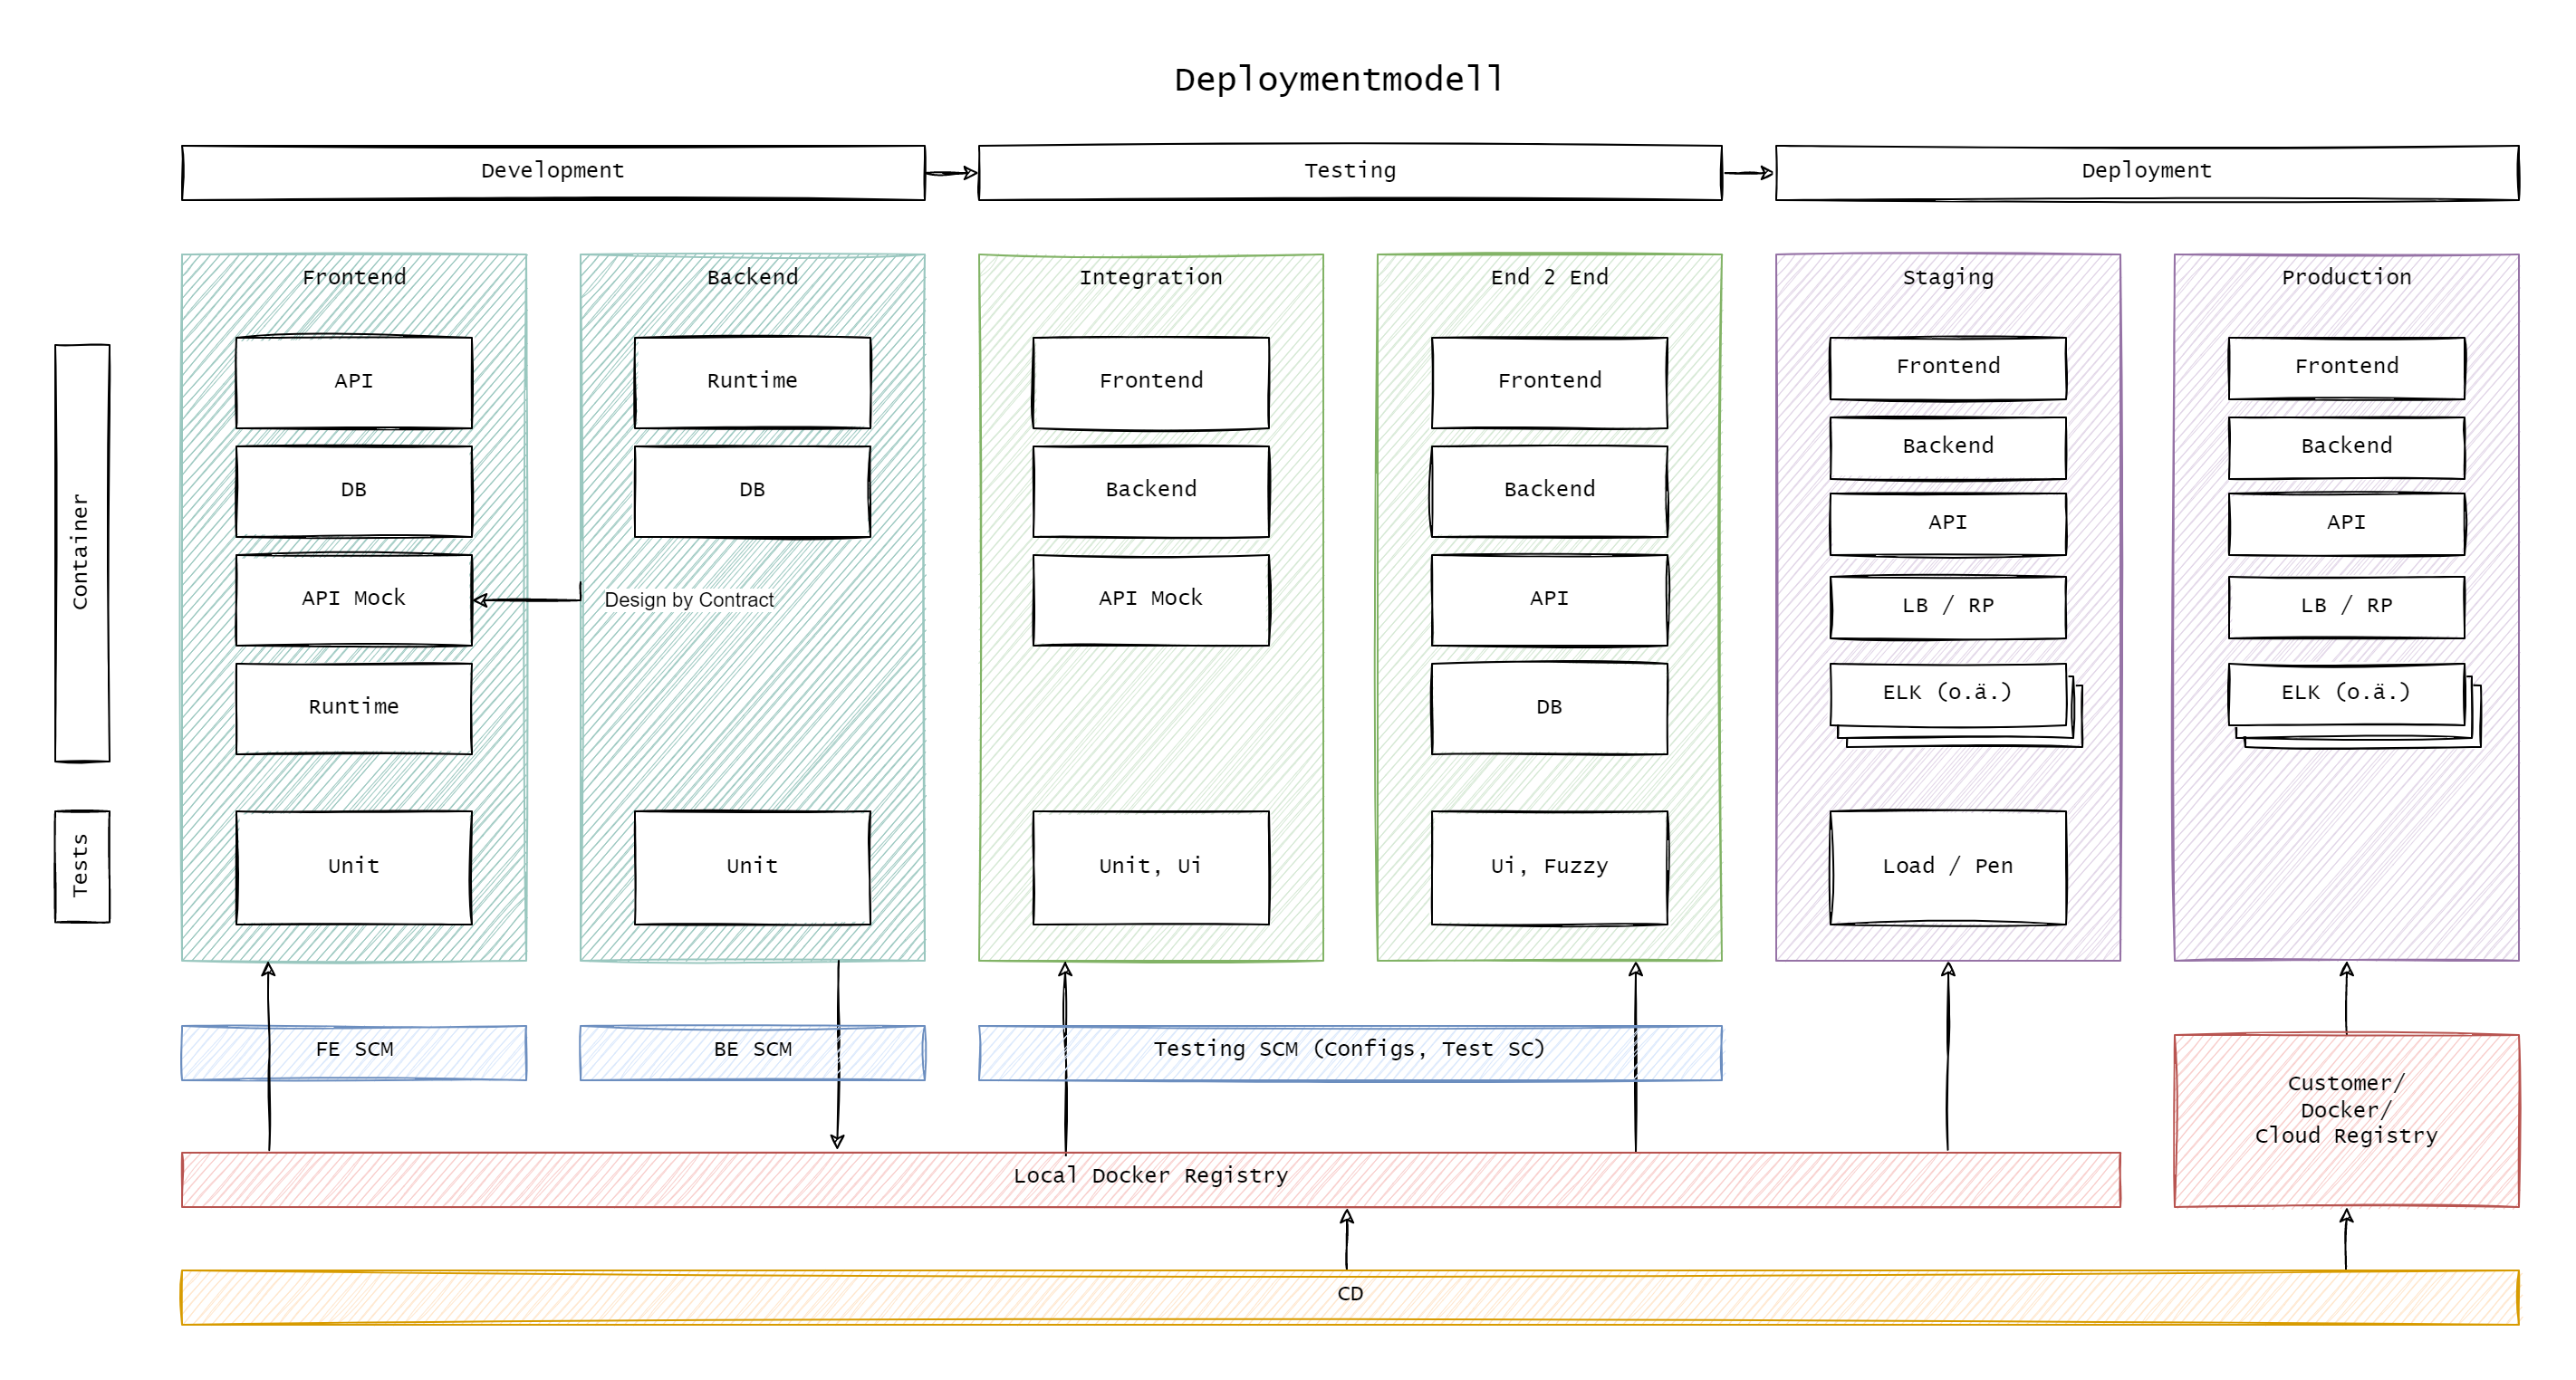
\includegraphics[width=\textwidth]{images/deployment.png}
  \caption{Deploymentdiagramm}
  \label{fig:deploymentdiagramm}
\end{figure}


\subsubsection{Umsetzung}
Entwicklung einer Web-API (mind. 6 Operationen bzw. Datenressourcen - ggf. CRUD) und eines korrespondierenden Client
\begin{itemize}
\item Berücksichtigen Sie in der Doku Analyse, Design, Implementierung und Test
\item Deployment (Installation) innerhalb der Laufzeitumgebung
\end{itemize}

Analyse: nee, Test nee

\paragraph{Design} \mbox{} \\
Komponentendiagramm, Deploymentdiagramm, 

\paragraph{Implementierung} \mbox{} \\
Blablabla

\subparagraph{Client} \mbox{} \\
Blablabla

\begin{lstlisting}[language=SQL,frame=single,caption=cargo.toml Datei zur Organisation der Abhängigkeiten in Rust,label=toml]

\end{lstlisting}


\begin{figure}[H]
\centering
  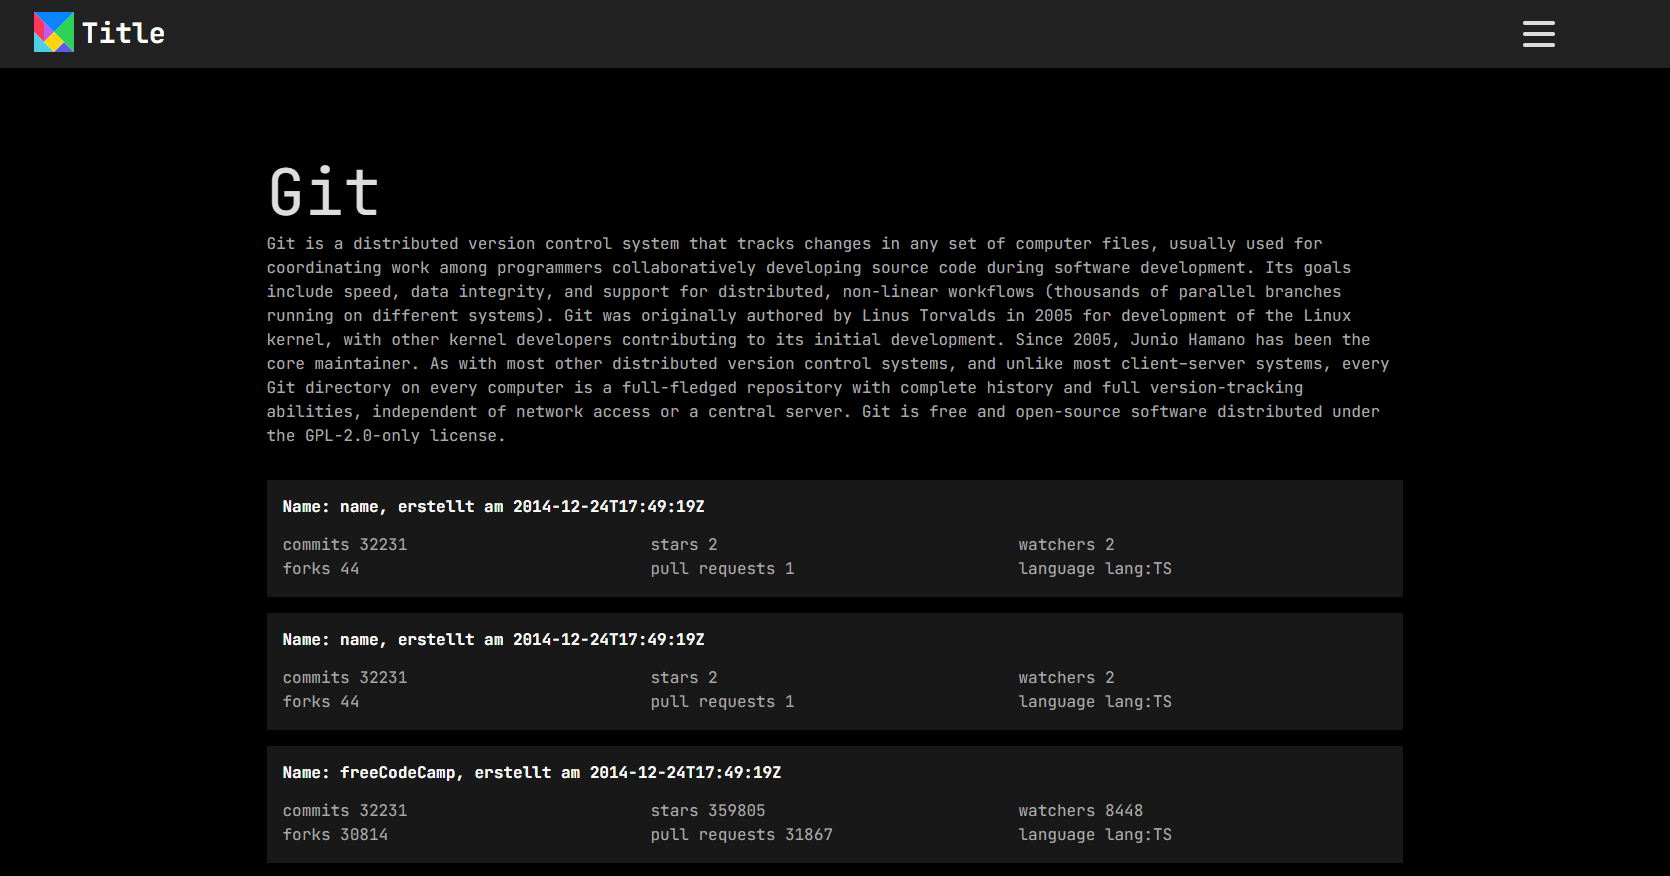
\includegraphics[width=\textwidth]{images/client.png}
  \caption{Screenshot des Clients}
  \label{fig:clientscreenshot}
\end{figure}

\subparagraph{REST API} \mbox{} \\
Blablabla

\begin{lstlisting}[language=SQL,frame=single,caption=cargo.toml Datei zur Organisation der Abhängigkeiten in Rust,label=toml]

\end{lstlisting}


\begin{figure}[H]
\centering
  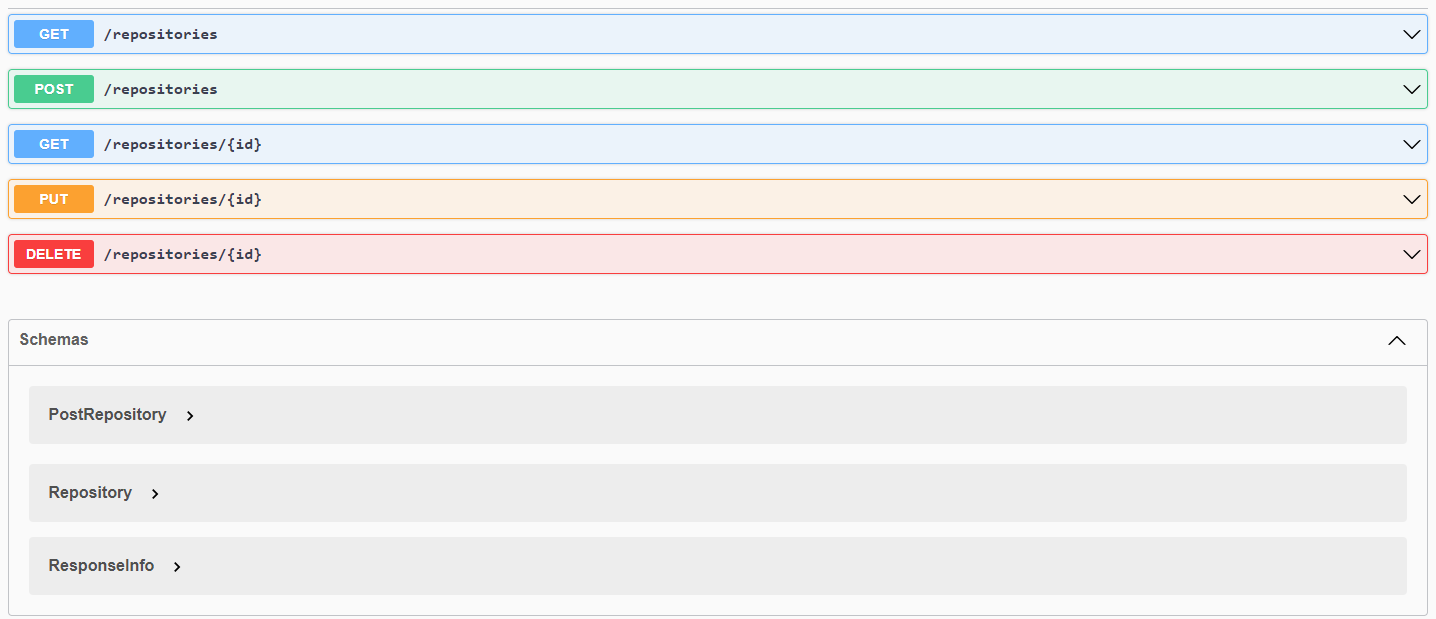
\includegraphics[width=\textwidth]{images/swagger.png}
  \caption{}
  \label{fig:apione}
\end{figure}


\subparagraph{Tests}  \mbox{} \\
Blablabla

\begin{figure}[H]
\centering
  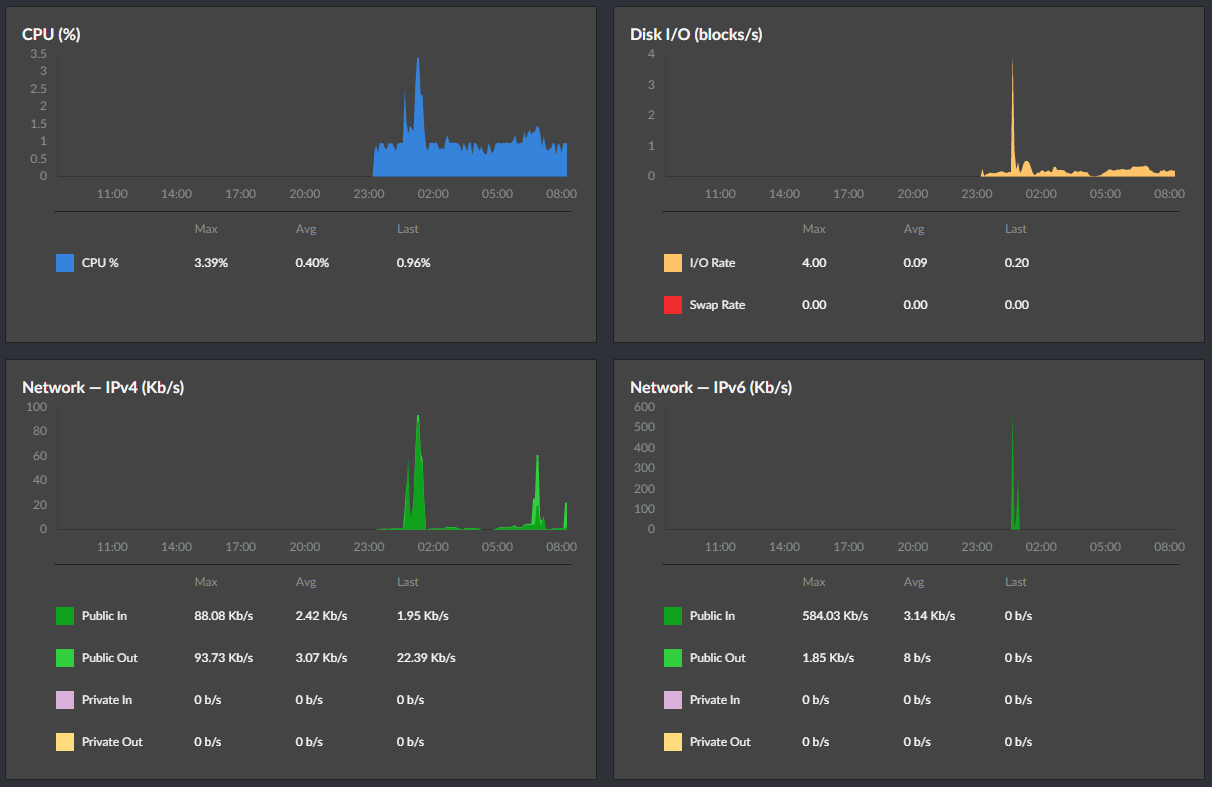
\includegraphics[width=\textwidth]{images/data2.png}
  \caption{}
  \label{fig:benchmarkone}
\end{figure}


\begin{figure}[H]
\centering
  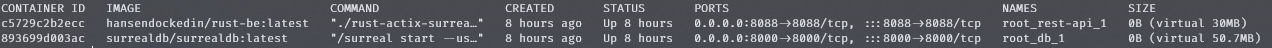
\includegraphics[width=\textwidth]{images/data4.png}
  \caption{}
  \label{fig:benchmarktwo}
\end{figure}


\begin{figure}[H]
\centering
  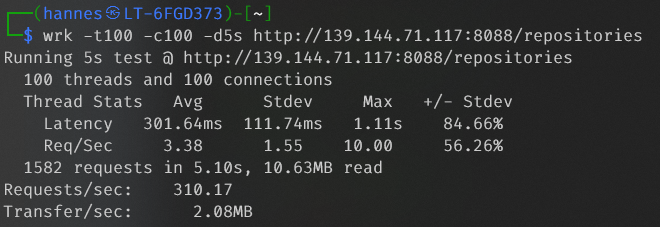
\includegraphics[width=250px]{images/data.png}
  \caption{}
  \label{fig:benchmarkthree}
\end{figure}


\begin{figure}[H]
\centering
  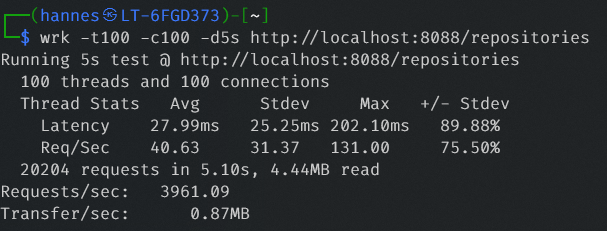
\includegraphics[width=250px]{images/data5.png}
  \caption{}
  \label{fig:benchmarkfour}
\end{figure}


\paragraph{Deployment} \mbox{} \\
 Für beide selbst entwickelten Services wird mit Hilfe von Dockerfiles (Listing \ref{deploymentone}) ein Image erstellt und aufs Dockerhub gepusht. In einem produktiven Szenario, insbesondere wenn der Code Closed Source ist, sollte stattdessen eine eigene Docker Registry verwendet werden. Die Schritte zur Öffentlichung sind jedoch bis auf den Host im Command docker push ... dieselben. 

\begin{lstlisting}[language=SQL,frame=single,caption=Dockerfile für die Erstellung des REST-API Images ,label=deploymentone]
FROM rust:1.60.0-bullseye AS build
WORKDIR /app
COPY . .
RUN cargo build --release
RUN mkdir -p /app/lib
RUN cp -LR $(ldd ./target/release/rust-actix-surreal-rest-api | grep "=>" | cut -d ' ' -f 3) /app/lib

FROM scratch AS app
WORKDIR /app
COPY --from=build /app/lib /app/lib
COPY --from=build /lib64/ld-linux-x86-64.so.2 /lib64/ld-linux-x86-64.so.2
COPY --from=build /app/target/release/rust-actix-surreal-rest-api rust-actix-surreal-rest-api
ENV LD_LIBRARY_PATH=/app/lib
ENTRYPOINT ["./rust-actix-surreal-rest-api"]
\end{lstlisting}

Auf dem Server, auf welchem die Services laufen sollen, muss ein Pull der Images erfolgen oder der Pfad zur Registry im docker-compose File angegeben sein, dann wird das Image automatisch bezogen. Die Ausführung von docker-compose up -d erstellt dann aus den Images die Container mit der dargestellten Konfiguration. Die virtuell erstellten Netzwerke in Docker (s. Listing \ref{deploymenttwo} in Zeile 11, 18 und 31) ermöglichen eine zusätzliche Kapselung, der einzig nach außen geöffnete Port ist im Beispiel 8080. In einer produktiven Umgebung wäre hier entweder noch ein weiterer Service in Form eines Reverse Proxys (z.B. nginx oder traefik) vorhanden, welcher über Port 443 erreichbar ist und über LetsEncrypt ein Zertifikat bezieht. Alternativ könnte auf dem Server direkt ein nginx Webserver bereitgestellt werden, Hauptsache die über HTTP erreichbaren Services sind in einem gekapselten Netzwerk nur über die Weiterleitung der Anfragen des Reverse Proxys erreichbar. 

\begin{lstlisting}[language=SQL,frame=single,caption=docker-compose.yml zur Bereitstellung des kompletten Stacks,label=deploymenttwo]
version : '3.8'
services:
  db:
    image: surrealdb/surrealdb:latest
    restart: always
    command: start --user root --pass root memory
    expose:
      - 8000
    volumes:
      - db:/var/lib/surrealdb/data
    networks:
      - backend

  rest-api:
    image: rust-actix-surreal-rest-api    
    expose: 
      - 8088
    networks:
      - backend
      - frontend
    depends_on:
      - db
    environment:
      - BASE_URL=http://db
      - CORS_ALLOW=http://localhost:8080
      
  client:
    image: rust-client    
    ports: 
      - '8080:8080'
    networks:
      - frontend
    depends_on:
      - rest-api
    environment:
      - SERVICE_URL=http://rest-api

networks:
  backend:
\end{lstlisting}

Die dargestellte Form des Deployments ermöglicht eine sehr schnelle Aktualisierung der Services. Der Veröffentlichung des neuen Images würde i.d.R. natürlich ein umfangreiches, automatisiertes Testing vorausgehen, das Image selbst ist dann das Artefakt. Die erneute Ausführung von docker-compose up -d würde dann ausschließlich die Container neu starten, für welche Änderungen der Images festgestellt wurden. Dies dauert maximal einige Sekunden. Um auch dies zu vermeiden wäre es mit wenigen Zeilen zusätzlicher Konfiguration möglich, die Container zu replizieren und nach Terminierung der Verbindung im Reverse Proxy dynamisch die Last zu verteilen. Der Reverse Proxy hat dann dementsprechend gleichzeitig die Funktion eines Loadbalancers. \\
Um den Rahmen nicht zu sprengen, haben wir kein Monitoring und Remote Logging realisiert, auch dies wäre jedoch durch die Nutzung von Docker einfach umzusetzen. Images, z.B. für den oft verwendeten ELK Stack oder alternativ die Kombination von Grafana und Prometheus, sind vorhanden und mit wenigen Anpassungen als weitere Services innerhalb der docker-compose File einsetzbar. Des weiteren würden die Services in einem produktiven Umfeld als Cluster auf physisch getrennten Systemen laufen.\\
Das Deployment kann auf jedem beliebigen Linuxserver erfolgen, auf dem Docker installiert ist. In unserem Fall haben wir Linode (Akamai) als IAAS Anbieter ausgewählt und die Anwendung auf einem Alpine Server mit 1GB RAM bereitgestellt. 


\subsubsection{Anbindung Datenbank} \label{anbindungdatenbank}
Originäre Verwendung eines DBMS (auch NoSQL) als Service-Schnittstelle
\begin{itemize}
\item Prototypisches Aufsetzen eines konkreten Datenbanksystems (ggf. Cloud)
\item Details der Konfiguration und Administration – ggf. Probleme
\item Eigene Kapselung mit Hilfe einer WSDL, Swagger oder GraphQL
\item Performanter Umgang mit XML/JSON-basierten Datenströmen
\end{itemize}

{[Sharp]C}
\begin{lstlisting}[language=bash,frame=single,caption=CLI Kommandos zur lokalen Installation der Datenbank für Windows\, Linux und macOS,label=dbinstall]
iwr https://windows.surrealdb.com -useb | iex
curl -sSf https://install.surrealdb.com | sh
brew install surrealdb/tap/surreal
\end{lstlisting}

\begin{lstlisting}[language=bash,frame=single,caption=CLI Kommando zur Übertragung der Daten aus der Datei in Listing \ref{sqldbone},label=dbsetup]
cat schemashort.sql | surreal sql --conn http://localhost:8000 --user root --pass root --ns base --db base
\end{lstlisting}


\begin{lstlisting}[language=SQL,frame=single,caption=Ausschnitt der sql Setupdatei,label=sqldbone]
INSERT INTO repository (name, stars_count, forks_count, watchers, pull_requests, primary_language, languages_used, commit_count, created_at, licence) VALUES ('react', 159266, 30464, 8497, 2911, lang:JavaScript, [lang:JavaScript, lang:HTML, lang:CSS], 5562, '2013-05-24T16:15:54Z', 'MIT License');
INSERT INTO repository (name, stars_count, forks_count, watchers, pull_requests, primary_language, languages_used, commit_count, created_at, licence) VALUES ('scikit-learn', 38327, 18225, 4968, 1701, lang:Python, [lang:Python, lang:Cython, lang:HTML, lang:CSS], 4085, '2010-01-10T09:58:52Z', 'BSD-3-Clause License');
INSERT INTO repository (name, stars_count, forks_count, watchers, pull_requests, primary_language, languages_used, commit_count, created_at, licence) VALUES ('angular', 68521, 24536, 6779, 2197, lang:TypeScript, [lang:TypeScript, lang:JavaScript, lang:HTML, lang:CSS], 4248, '2014-09-18T16:12:01Z', 'MIT License');
\end{lstlisting}



\newpage
\section{Übung 4d: Sicherheit von Web APIs}
\subsection{Sicherheitsrisiken in Verbindung mit dem HTTP Protokoll}
\begin{itemize}
\item Beschreiben Sie stichpunktartig die Eigenschaften von TLS (SSL) in Verbindung mit HTTPS
\item Welche Verfahren zur Authentifizierung können im Rahmen des HTTP Protokolls \textbf{direkt} verwendet werden? Gehen Sie auf Stärken und Schwächen ein
\item Authentifizierungs- und Benutzerinformationen werden bei Webanwendungen häufig mit Hilfe von Cookies übertragen. Gehen Sie auf die damit einhergehenden Nachteile ein. 
\end{itemize}

\subsubsection{HTTPS und TLS}
HTTP Eigenschaften:
\begin{itemize}
\item ist das Standardprotokoll für die Internetkommunikation
\item arbeitet nach dem Client Server Modell
\item nutzt TCP
\item hat zwei Typen: non-persistent (weniger Overhead, einmalige Verbindung, wird nicht aufrechterhalten) und persistent (Verbindung wird nach Aufbau aufrechterhalten, s. \ref{sockets})
\item funktioniert über Request und Response Message
\item Benutzer- und Serverstatus werden über Cookies aufrechterhalten
\item Webcache kann Geschwindigkeit erhöhen (lokal im Browser oder serverseitig auf Proxy), Response ist 304 (conditional GET)
\item HTTPS (S steht für secure) ist eine Erweiterung von HTTP
\end{itemize}

TLS Eigenschaften: (Wiki)
\begin{itemize}
\item Nachfolger von SSL, steht für Transport Layer Security
\item Verbindung zu HTTPS: kommt im TCP/IP Stack zwischen Transport und Anwendungsebene zum Einsatz und wird i.d.R. zusätzlich zum TCP Protokoll eingesetzt. 
\item ermöglicht eine Ende zu Ende Verschlüsselung von Data in Transit (und ist deshalb z.B. bei Mails durch zusätzliche Teilnehmer zwischen den ``Enden'' nur eingeschränkt sicher)
\item Im TLS Handshake findet ein sicherer Schlüsselaustausch und eine Authentifizierung statt.
\item Für den Schlüsselaustausch sind in den älteren TLS-Versionen verschiedene Algorithmen mit unterschiedlichen Sicherheitsgarantien im Einsatz. Die neueste Version TLS 1.3 verwendet allerdings nur noch das Diffie-Hellman-Schlüsselaustausch Protokoll (DHE oder ECDHE) auf Basis elliptischer Kurven.
\item Dabei wird für jede Verbindung ein neuer Sitzungsschlüssel (Session Key) ausgehandelt. Da dies ohne Verwendung eines Langzeitschlüssels geschieht, erreicht TLS 1.3 Perfect Forward Secrecy.
\item Alle TLS-Handshakes verwenden eine asymmetrische Kryptographie (öffentlicher und privater Schlüssel), aber nicht alle nutzen den privaten Schlüssel beim Generieren von Sitzungsschlüsseln.
\end{itemize}

Vorteile TLS (1.3):
TLS 1.3 hat die Unterstützung für ältere, weniger sichere kryptografische Features eingestellt und unter anderem TLS-Handshakes schneller gemacht. Die Hauptvorteile von TLS 1.3 gegenüber TLS 1.2 sind schnellere Geschwindigkeiten und verbesserte Sicherheit. TLS und verschlüsselte Verbindungen erzeugen naturgemäß einen Overhead bei der Übertragung. HTTP / 2 hat bei diesem Problem durch die Verringerung der Schritte beim Aufbau der TCP Verbindung geholfen, aber TLS 1.3 beschleunigt verschlüsselte Verbindungen durch Funktionen wie TLS false start und Zero Round Trip Time (0-RTT) noch weiter. Die Einführung elliptischer Kurven verbessert zudem bei gleicher Schlüssellänge die Sicherheit und vermeidet beispielsweise Angriffe wie LogJam, die auf dem Number field sieve Algorithmus basieren (welcher die Tatsache ausnutzt, dass immer dieselbe Primzahl verwendet wird). Auch export-grade Funktionalitäten (welche demselben Angriff zugrunde lagen) sind in TLS 1.3 nicht mehr eingebaut.

\subsubsection{Authentifizierungmöglichkeiten HTTP(S)}
Es gibt mehrere Möglichkeiten, Benutzer (Clients) im Rahmen des HTTP-Protokolls zu authentifizieren. Verbreitet sind (Wiki, ssl.com):
\begin{itemize}
\item Basic Authentication: Die Basic Authentication (Basisauthentifizierung) wird seit 2015 durch RFC 7617 spezifiziert und ist eine häufig verwendete Art der HTTP-Authentifizierung. Der Webserver fordert mit Eingabe von Benutzername und Passwort eine Authentifizierung an. Ein Vorteil der Basic Authentication ist ihre Einfachheit in der Implementierung. Ein Nachteil ist, dass die Anmeldeinformationen im Klartext übertragen werden und daher leicht abgefangen werden können. Deshalb sollte diese Methode nur für den Hobbybereich eingesetzt werden.
\item Digest Access Authentication: Die Hashwertauthentifizierung ist ein Verfahren, das die Basic-Authentifizierung ersetzen soll(te). Der Server sendet eine Zeichenfolge zufälliger Daten, auch Nonce genannt, als Challenge an den Client. Der Client reagiert mit einem Hash, der neben anderen Informationen den Benutzernamen, das Kennwort und die Nonce enthält. Die Digest Access Authentication bietet mehr Sicherheit als die Basic Authentication, da sie einen Hash verwendet und somit die Anmeldeinformationen nicht im Klartext übertragen werden.
\end{itemize}

Weitere Verfahren, die im Zusammenhang mit HTTPS eingesetzt werden, sind nicht den direkten Verfahren zuzurechnen, weil sie alle eine dritte Instanz hinzuziehen müssen (Validierung Zertifikate über PKI, Authorisierungs- bzw. Authentifizierungsprüfung über Drittanbieter bei OAuth2 und OIDC).

\subsubsection{Cookies}
\paragraph{Begriff}
Cookies sind kleine Textdateien, die von einer Webseite im Internetbrowser eines Nutzers gespeichert werden können. Sie dienen dazu, Informationen über den Nutzer und seine Interaktionen mit der Webseite zu speichern. \\
Cookies können nützlich sein, indem sie beispielsweise Einstellungen im Webbrowser abspeichern oder dafür sorgen, dass ein Warenkorb beim Online-Shopping zu einem späteren Zeitpunkt wieder aufgerufen werden kann. Sie können auch dazu verwendet werden, das Surfverhalten von Nutzern im Internet über einen längeren Zeitraum zu verfolgen und detaillierte Nutzerprofile anzulegen (was eher aus Sicht des Betreibers ein Vorteil ist...). \\
Grundsätzlich werden zwei Arten von Cookies unterschieden: technisch notwendige und technisch nicht notwendige Cookies. Technisch notwendige Cookies sind für das Funktionieren der Webseite notwendig, während technisch nicht notwendige Cookies für Zwecke wie das Verfolgen des Surfverhaltens verwendet werden können. \\
Es ist zwar möglich, eine Webseite ohne Cookies zu betreiben, allerdings kann dies zu Einschränkungen in der Funktionalität führen. Beispielsweise müssten Nutzer bei jedem Besuch der Webseite erneut ihre Einstellungen vornehmen oder sich erneut anmelden. Sofern jedoch eine Persistierung von Nutzerdaten nicht notwendig ist, z.B. bei statischen, rein informativen Seiten, kann auf Cookies verzichtet werden (was oft nicht passiert, weil durch den Einsatz von Tracking, eingebetteten Webfonts usw. auch auf solchen Seiten, Cookies gesetzt werden). Dabei sollte jedoch zwischen tendenziell unkritischen Sessioncookies, die lokal und verschlüsselt gespeichert werden und Trackingcookies, welche übertragen werden, unterschieden werden.   \\  
Ein großer Nachteil von Cookies ist mit ihnen einhergehende Sicherheitsrisiko. Da sie Informationen über den Nutzer und seine Interaktionen mit der Webseite speichern, können sie von Dritten abgefangen und missbraucht werden.

\paragraph{Sicherheitsrisiken}
Cookie Poisoning, XSS, Cookiethief


\subsection{Möglichkeiten zur Risikominderung}
\subsubsection{OWASP}
Machen Sie sich mit den OWASP Top 10 API Security Risiken vertraut
\begin{itemize}
\item Gehen Sie für 5 Sicherheitslücken auf entwicklerseitige oder betriebliche Möglichkeiten zur Verminderung bzw. Abmilderung ein

\begin{lstlisting}[language={[Sharp]C},frame=single,caption=,label=owasponebad]
[HttpGet("{id}")]
public async Task<IActionResult<User>> GetUser(int id)
{
    var user = await _context.Users.FindAsync(id);
    return Ok(user ?? NotFound());
}
\end{lstlisting}

\begin{lstlisting}[language={[Sharp]C},frame=single,caption=,label=owasponegood]
[HttpGet("{id}")]
[Authorize(Roles = "admin")]
public async Task<IActionResult<Item>> GetItem(Guid id)
{
    // Verify if the user has access to the requested resource by checking the user's authorization
    // against the resource's owner or other access control policies.
    var currentUser = HttpContext.User;
    var user = await _context.Users
        .Where(i => i.Id == id && i.OwnerId == currentUser.FindFirstValue(ClaimTypes.NameIdentifier))
        .SingleOrDefaultAsync();

    return Ok(user ?? NotFound());
}
\end{lstlisting}

\begin{lstlisting}[language={[Sharp]C},frame=single,caption=,label=owasponebad]
\end{lstlisting}

\begin{lstlisting}[language={[Sharp]C},frame=single,caption=,label=owasponebad]
\end{lstlisting}

\begin{lstlisting}[language={[Sharp]C},frame=single,caption=,label=owasponebad]
\end{lstlisting}

\begin{lstlisting}[language={[Sharp]C},frame=single,caption=,label=owasponebad]
\end{lstlisting}



\item Gehen Sie für 2 Sicherheitslücken auf die Möglichkeiten von Tests zur Aufdeckung potentieller Schwachstellen ein.
\end{itemize}

\subsubsection{OAuth 2 und OIDC}
Analysieren Sie die grundlegende Arbeitsweise von OAuth2
\begin{itemize}
\item Welche grundlegenden Rollen werden in OAuth2 unterscheiden?
\item Welche Zusammenhänge bestehen zwischen OAuth2 und OIDC?
\end{itemize}

\subsection{Praktische Anwendung von OAuth2}
\subsubsection{Testwerkzeuge}
Verwenden Sie ein Testwerkzeug zur Nutzung von Web APIs und beschreiben Sie exakt die Schritte und Konfigurationen von mindestens 3 OAuth2 konformen Funktionsaufrufen (request), sie deren erhaltenen Antworten (response)

\subsubsection{Implementierung}
Gehen Sie auf die Möglichkeiten einer programmiertechnischen Einbindung von OAuth2 konformen Aufrufen innerhalb der Programmiersprache Java oder ggfs. auch JavaScript ein. 
\begin{itemize}
\item Voraussetzungen dokumentieren (genutzte APIs)
\item prototypische Verwendung mit Hilfe eines lauffähigen Quellcodefragments
\item Test des entwickelten Prototypen, d.h. OAuth2 Zugriff auf Web-APIs
\end{itemize}

\newpage

\bibliographystyle{te}

\bibliography{citation}

\end{document}